\section{Experiments}
\label{sec:experiments}

To show the wide applicability of Categorical Normalizing Flows, we perform experiments on sets, graphs, and language modeling. 
Our goal is to investigate whether Categorical Normalizing Flows can accurately model categorical distributions despite modeling a lower bound, and what flexibility of the encoding distributions is needed for that.
Furthermore, we compare our method to baselines such as Discrete Normalizing Flows \cite{TranDiscreteFlows} and variational dequantization \cite{Flow++}. 

We study the application of Categorical Normalizing Flows on graphs on two tasks: graph coloring and molecule generation. 
On graph coloring, we examine the effect of different node orderings in autoregressive models and compare their performance to the permutation-invariant GraphCNF.
Meanwhile, molecule generation resembles a complex modeling task with various categorical node and edge attributes.
Also, there has been recent work on applying normalizing flows on molecule generation which serve as a comparison to GraphCNF and show the effect of our architectural design choices \cite{GraphNVP, GraphAF}.
A final discussion of the findings in all experiments and an additional analysis is provided in Section~\ref{sec:experiments_discussion}.

The normalizing flows we use in our experiments consist of a sequence of logistic mixture coupling layers proposed by \citet{Flow++} which map a mixture of logistic distributions back into a single mode. 
As mentioned before, this is particularly of interest for our proposed encoding strategy as its simplest implementation is based on a logistic mixture model.
Before each coupling layer, we follow current standard techniques and include an activation normalization layer and invertible 1x1 convolution \cite{Glow}.  
For full reproducibility, we outline each experiment's hyperparameter details in Appendix~\ref{sec:appendix_hyperparams}, and publish our code\footnote{Our code can be found at \href{https://github.com/phlippe/CategoricalNF}{https://github.com/phlippe/CategoricalNF}}.

\begin{figure}[ht!]
    \centering
    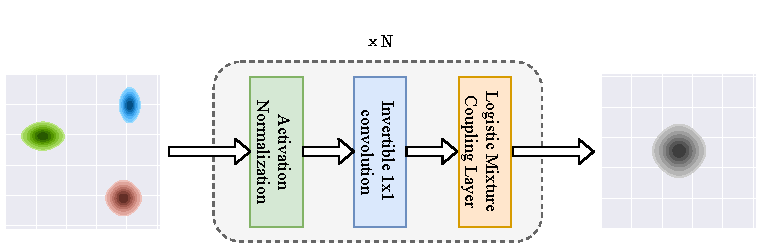
\includegraphics[width=0.75\textwidth]{figures/experiments_figures/flow_template_overview.pdf}
    \caption[Flow architecture in experiments]{Overview of the general flow architecture used in our experiments. We apply a sequence of activation normalization, invertible 1x1 convolution and logistic mixture coupling layer to map the categorical encoding (left) to a logistic base distribution (right). In case of GraphCNF, we use this sequence of flow layers within the three steps $f_1$, $f_2$ and $f_3$.}
    \label{fig:experiments_flow_template_overview}
\end{figure}


\subsection{Set modeling}
\label{sec:experiments_set_modeling}

\paragraph{Task} Sets have the unique property of being a collection of elements with no specific order. 
In order to evaluate how well different normalizing flows can model categorical distributions on sets, we create two toy datasets with a known data likelihood:  \textit{set shuffling} and \textit{set summation}. 
In set shuffling, we model a set of $N$ categorical variables each having one out of $N$ categories. 
However, each category has to appear exactly once in the set. 
Taking for instance $N=4$, we consider the set $\{1,2,3,4\}$.
Although the dataset consists of a single set, this set represents $N!$ possible assignments that need to be modeled. 
For the second toy dataset, set summation, we again consider a set of size $N$ with $N$ categories, but those categories represent the actual integers $1,2,...,N$. 
The task is to model those sets for which the sum of all elements is an arbitrary number, $L$. 
In contrast to the shuffling dataset, the data is ordinal in set summation, which we initially expected to help dequantization methods. 
In our experiments, we used $N=16$ for both datasets and $L=42$ for the summing dataset which gave us about 2000 different sets in the dataset.
For both datasets, we can compute the true likelihood in bits per element by determining the number of possible permutations for all instances together, denoted by $M$, and dividing its overall log-likelihood by the sequence length: $(\log_2 M)/N$. 

\paragraph{Models} We compare Categorical Normalizing Flows to applying variational dequantization \cite{Flow++}, Latent Normalizing Flows \cite{SemiDiscreteNFSequence} and Discrete Normalizing Flows by \citet{TranDiscreteFlows} with a factorized prior. 
In Categorical Normalizing Flows, we use a latent dimensionality of $d=4$ for each categorical variable and apply a channel mask making the flow permutation-invariant to its inputs.
While Latent Normalizing Flows can follow this setup as well, variational dequantization and Discrete NFs have to use a checkboard mask, i.e. masking every other element of the sequence, since they rely on a single dimension per discrete variable. Thus, these flows are sensitive to the order in the set.
For a fair comparison, all flows use the same setup of 8 coupling layers with a 2-layer transformer \cite{AttentionIsAllYouNeed} excluding the positional encoding. 
% We explicitly do not use positional encoding as commonly applied in transformers to maintain the permutation invariance of the data. 
Besides, we vary the encoding distribution in Categorical Normalizing Flows and compare a mixture model, linear flows, and variational encoding.
The Latent Normalizing Flows use a 2-layer transformer to determine the mean and scale of the logistic encoding distribution, and a second transformer network as decoder.

\begin{table}[t!]
	\caption[Results on set modeling]{Results on set modeling. Metric used is bits per categorical variable (dimension). The standard deviation across three seeds is reported next to the average of the models.}
	\label{tab:result_table_sets}
	\centering
	\begin{tabular}{lccc}
		\toprule
		\textbf{Model} & \textbf{Set shuffling} & \textbf{Set summation} \\
		\midrule
		Discrete NF \cite{TranDiscreteFlows} & $3.87$ \footnotesize{$\pm0.04$} & $2.51$ \footnotesize{$\pm0.00$}\\
		Variational Dequant. \cite{Flow++} & $3.01$ \footnotesize{$\pm0.02$} & $2.29$ \footnotesize{$\pm0.01$}\\
		Latent NF \cite{SemiDiscreteNFSequence} & $\bm{2.78}$  \footnotesize{$\pm0.00$} & $2.26$ \footnotesize{$\pm0.01$}\\[4pt]
		CNF $+$ Mixture model & $\bm{2.78}$ \footnotesize{$\pm0.00$} & $\bm{2.24}$  \footnotesize{$\pm0.00$}\\
		CNF $+$ Linear flows & $\bm{2.78}$ \footnotesize{$\pm0.00$} & $2.25$ \footnotesize{$\pm0.00$}\\
		CNF $+$ Variational Encoding & $2.79$ \footnotesize{$\pm0.01$} & $2.25$ \footnotesize{$\pm0.01$}\\
		\midrule 
		%Unigram & $4.00$bpd & $2.51$bpd \\
		Optimal & $2.77$ & $2.24$ \\
		\bottomrule
	\end{tabular}
\end{table}

\paragraph{Results} Our results are summarized in Table~\ref{tab:result_table_sets}. 
On both datasets, Categorical Normalizing Flows achieve close-to-optimal performance with a maximum offset of $0.01$bpd. 
This shows that although we model a lower bound in continuous space, Categorical Normalizing Flows can model discrete distributions precisely. 
Interestingly, representing the categories by a simple mixture model is sufficient for achieving these results, and more complex encoding distributions did not result in improvements. 
We observed the same trend in experiments with more complex relations between categories, such as on the graph and language modeling. 
This is presumably because of both the coupling layers and the prior distribution rest upon logistic distributions as well.
Modeling a different encoding distribution would require additional transformations inside the flow to map them back to a logistic base distribution.
This hypothesis is supported when taking a closer look at the distributions learned by linear flows and the variational encoding.
We experienced that both have fallen back to a logistic distribution per category despite being able to model much more complex distributions.
Hence, we can conclude that encoding categorical variables by a simple mixture model is indeed sufficiently powerful and efficient.

Introducing dependencies between categorical variables during decoding, as done in Latent Normalizing Flows, also shows to achieve good performance although slightly lower on set summation.
On set shuffling, the encoding parameters are constant since we only learn a single set such that the input to the encoder is always the same. 
Thus, the model effectively falls back to a mixture model.
To train Latent NFs on set summation, weighting the reconstruction error of the decoder significantly higher than the prior in the beginning of the training showed to be crucial.
In this phase, the decoder learns to be deterministic and the prior is complex enough to model the latent space consecutively.
This weighting is similar to the KL scheduling that is commonly done in VAEs and follow \citet{SemiDiscreteNFSequence} original setup.
Nevertheless, it should be kept in mind that Latent NFs model a lower bound which also attributes to the slightly higher bits per dimension score.

Meanwhile, the variational dequantization obtains a considerably worse performance on the shuffling dataset, underlining that dequantization methods cannot represent categorical data well. 
In set summation, where the categories represented integers, we see a closer score, although it is still performing considerably worse than Categorical Normalizing Flows. 
Discrete Normalizing Flows was not able to model the categorical distributions well in our experiments, mostly due to notable optimization issues we experienced. 
Following the hyperparameter setting of \citet{TranDiscreteFlows}, we experienced that discrete flows got stuck in local optima, and gradients vanished due to approximations of discrete operations. 
In contrast, Categorical Normalizing Flows is not suffering from such gradient issues by modeling the transformations in continuous space.

\subsection{Graph coloring}
\label{sec:experiments_graph_coloring}

\paragraph{Task} Graph coloring is a well-known combinatorial problem which finds use in many applications \cite{bondy1976graph, GraphColoringDL, GraphColoringApplications}. 
Given a graph $\mathcal{G}$, the task is to assign each node one out of $K$ colors. However, two adjacent nodes are not allowed to have the same color. 
Consequently, there are a limited number of valid colorings for each graph. 
Modeling the distribution of these solutions to arbitrary graphs is a challenging task as it has been shown to be NP-complete \cite{bondy1976graph}. 
With this experiment, we aim to verify that assuming an order can have a significant influence on autoregressive graph models and that the permutation-invariant GraphCNF can achieve similar performance to the best autoregressive order.

\paragraph{Dataset} To train models on modeling such a distribution, we generate a dataset of graph colorings by randomly sampling a graph and using an SAT solver 
%\footnote{We have used the following solver from the OR-Tools library in python: \href{https://developers.google.com/optimization/cp/cp_solver}{https://developers.google.com/optimization/cp/cp\_solver}} 
for finding one valid coloring assignment. In our experiments, we focus on the 3-color problem meaning that a graph has to be colored using $K=3$ colors. A detailed description of the dataset generation can be found in Appendix
~\ref{sec:appendix_hyperparams_graph_coloring}. We create two dataset versions, one with graphs of size $10\leq|V|\leq20$ and another with $25\leq|V|\leq50$, to further investigate the effect of complexity as larger graphs are commonly harder to solve. Overall, we use 200k and 450k examples for training and evaluate on a test set with 25k previously unseen graphs. We visualize examples of the datasets in Figure~\ref{fig:experiments_graph_coloring_examples}.

\begin{figure}[b!]
    \centering
    \setlength{\tabcolsep}{20pt}
    \begin{tabular}{cc}
        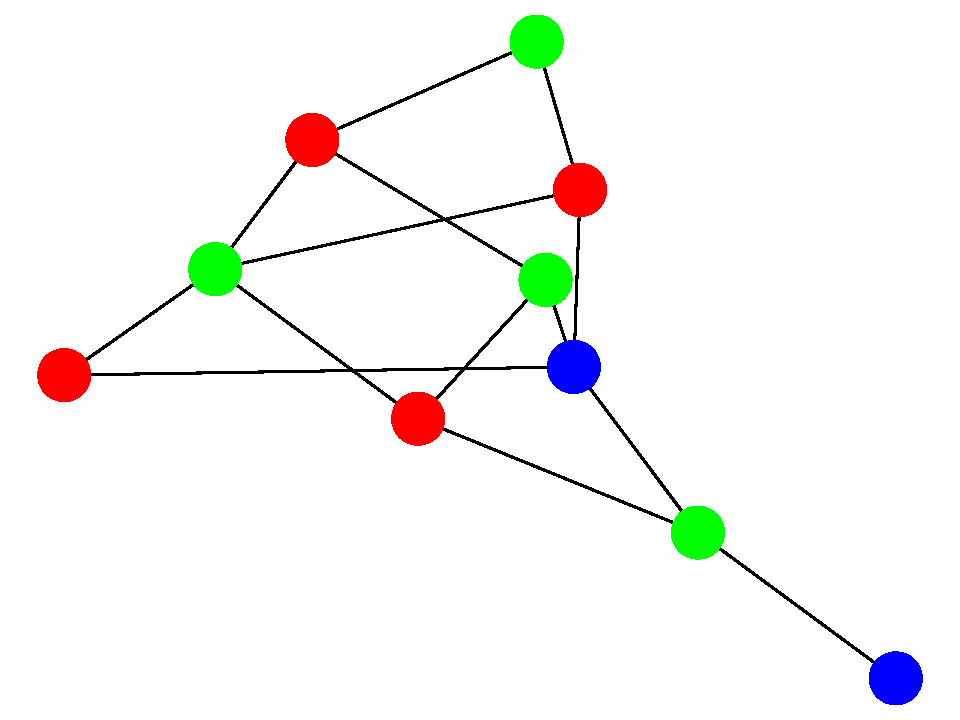
\includegraphics[height=3cm]{figures/experiments_figures/dataset_figures/graph_coloring/exmp_tiny_0.pdf} &  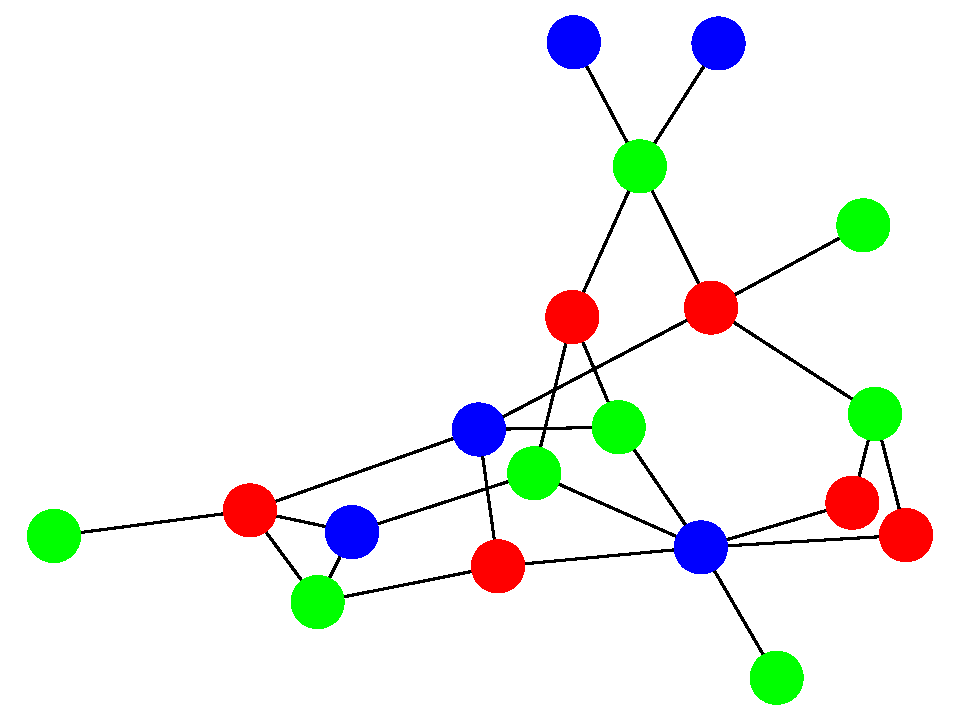
\includegraphics[height=3cm]{figures/experiments_figures/dataset_figures/graph_coloring/exmp_tiny_9.pdf}\\
        (a)  $|V|=10$ & (b)  $|V|=19$\\[4pt]
        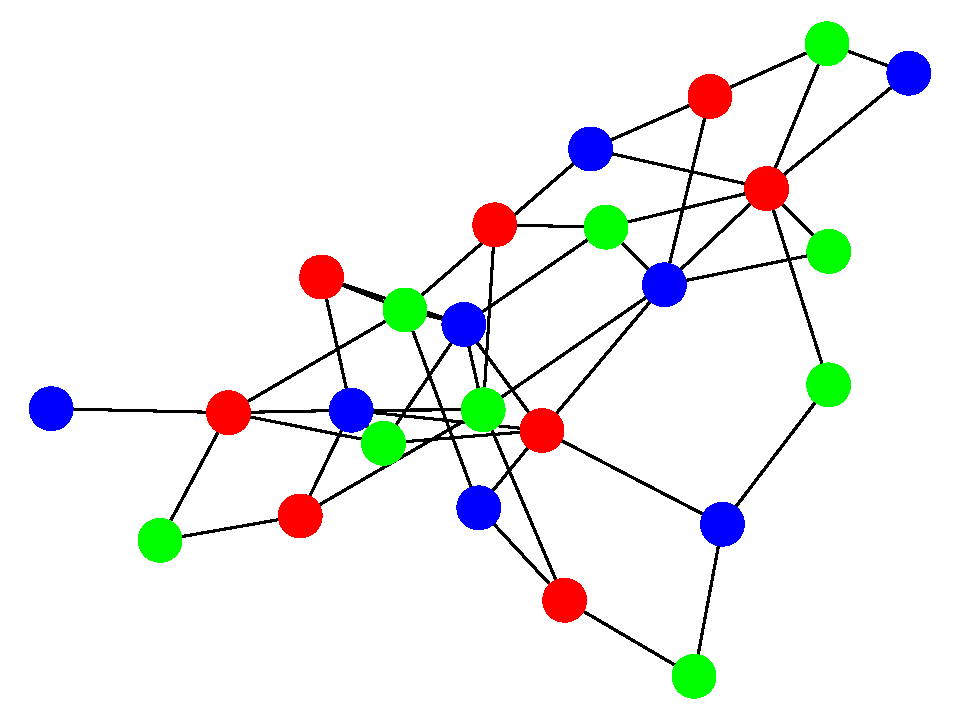
\includegraphics[height=4cm]{figures/experiments_figures/dataset_figures/graph_coloring/exmp_large_4.pdf} & 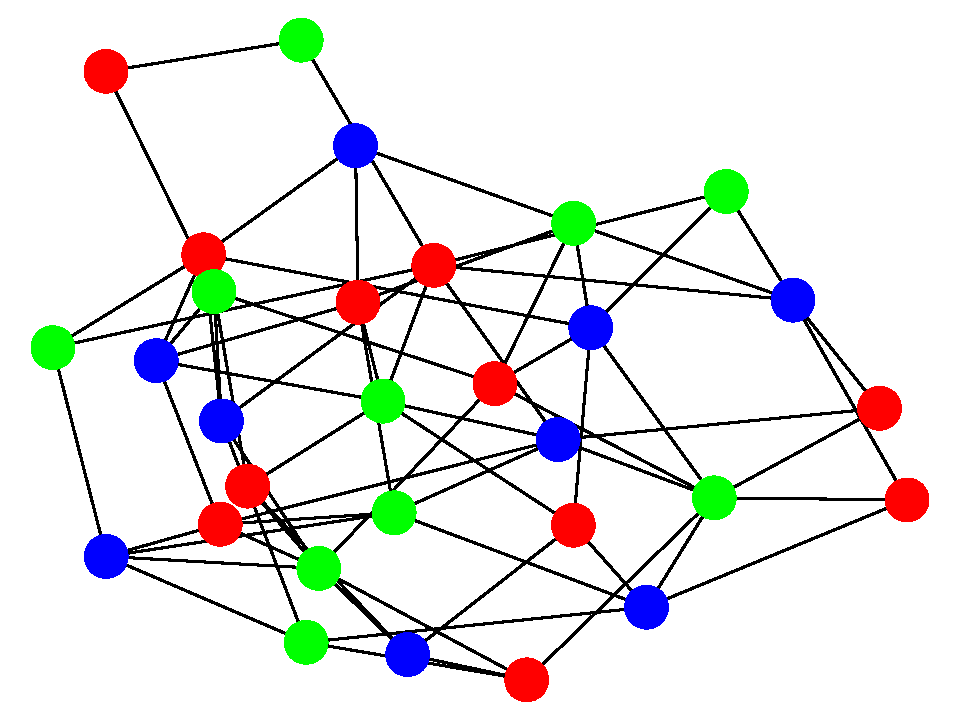
\includegraphics[height=4cm]{figures/experiments_figures/dataset_figures/graph_coloring/exmp_large_9.pdf}\\
        (c)  $|V|=25$ & (d)  $|V|=30$\\
    \end{tabular}
    \caption[Examples of graph coloring]{Examples of valid graph color assignments from the dataset (best viewed in color). Due to the graph sizes and dense adjacency matrices, edges can be occluded or cluttered in (c) and (d).}
    \label{fig:experiments_graph_coloring_examples}
\end{figure}

\paragraph{Models} We compare GraphCNF to a variational autoencoder and an autoregressive prediction model which generates one node at a time. 
Considering graph coloring does not require edge generation, we only use the first step of GraphCNF's three-step generation. 
For all models, we apply the same Graph Attention network \cite{GraphAttentionNetwork}. 
Note that due to the different sampling techniques, we cannot guarantee a fully fair comparison in terms of number of parameters and layer depth across models.
For instance, Normalizing Flows require considerably more parameters than autoregressive models although being much faster to sample from.
Thus, we tried to balance the complexity of the model and the sampling time when designing the models. 
More details can be found in Appendix~\ref{sec:appendix_hyperparams_graph_coloring}.

As autoregressive models require a manually prescribed node order, we compare the following: a \emph{random} ordering per graph, \textit{largest\_first} which is inspired by heuristics of automated theorem provers that start from the nodes with the most connections, and \textit{smallest\_first}, where we reverse the order of the previous heuristic. 

\paragraph{Metrics} We evaluate the models based on two metrics. First, the likelihood of the test dataset is measured by bits per node. A low likelihood shows the generalization property of the model to new graphs, and the coverage of all possible solutions for a graph by the model. 
The second metric we use is \textit{validity}. 
Validity is measured by randomly sampling a color assignment from the model for each graph in the test dataset, and reporting the percentage of samples which were a valid solution by having different colors for all adjacent nodes. 
Therefore, this metric represents the modeled discrete distribution and its closeness to the learned rules. 
Note that we sample with a temperature value of $T=1.0$, meaning that we sample from the original softmax distribution in autoregressive models and the original prior in normalizing flows and variational autoencoders. 
A lower temperature value reduces the variance during sampling and biases the samples towards the most likely values.
Nonetheless, we do not lower it here because we want to test the full discrete distribution of the model.

\begin{table}[t]
	\caption[Results on graph coloring]{Results on the graph coloring problem. The column \textit{time} shows the average time for the different models needed to sample a batch of 128 graph coloring assignments on a NVIDIA TitanRTX. In the last row, we report the results of GraphCNF with affine coupling layers. The standard deviation was omitted for readability and can be found in the appendix, Table~\ref{tab:appendix_results_graph_coloring}.}
	\label{tab:result_table_graph_coloring}
	\centering
	\begin{tabular*}{\columnwidth}{@{\extracolsep{\fill}}l*{6}{c}}
		\toprule
		& \multicolumn{3}{c}{$10\leq|V|\leq20$} & \multicolumn{3}{c}{$25\leq|V|\leq50$} \\
		\cmidrule{2-4} \cmidrule{5-7}
		\textbf{Method} & \textbf{Validity} & \textbf{Bits per node} & \textbf{Time} & \textbf{Validity} & \textbf{Bits per node} & \textbf{Time}  \\
		\midrule
		VAE & $44.95\%$ & $0.84$bpd & $0.05$s & $7.75\%$ & $0.64$bpd & $0.10$s \\
		% Autoregressive & & & $0.69$s & & & $2.88$s \\
		% - Smallest\_first & $76.86\%$ & $0.73$bpd & & $32.27\%$ & $0.50$bpd &\\
		% - Random & $88.62\%$ & $0.70$bpd & & $49.28\%$ & $0.46$bpd &\\
		% - Largest\_first & $93.41\%$ & $0.68$bpd & & $\bm{71.32\%}$ & $\bm{0.43}$bpd &\\
		RNN$+$Smallest\_first & $76.86\%$ & $0.73$bpd & $0.69$s & $32.27\%$ & $0.50$bpd & $2.88$s\\
		RNN$+$Random & $88.62\%$ & $0.70$bpd & $0.69$s & $49.28\%$ & $0.46$bpd & $2.88$s\\
		RNN$+$Largest\_first & $93.41\%$ & $0.68$bpd & $0.69$s & $\bm{71.32\%}$ & $\bm{0.43}$bpd & $2.88$s\\
		\midrule
		GraphCNF & $\bm{94.56\%}$ & $\bm{0.67}$bpd & $0.28$s & $66.80\%$ & $0.45$bpd & $0.54s$\\
		$-$ Affine & $93.90\%$ & $0.69$bpd & $0.12$s & $65.78\%$ & $0.47$bpd & $0.35$s\\
		\bottomrule
	\end{tabular*}
\end{table}

\paragraph{Results} Table~\ref{tab:result_table_graph_coloring} summarizes the results. 
As we initially expected, the node order has a significant effect on the autoregressive model's performance which becomes the clearest in terms of validity. 
While sorting the nodes according to smallest\_first leads to only $32\%$ valid solutions on the large dataset, reversing the order simplifies the task for the model such that it generates more than twice as many valid color assignments. 
The ordering also shows to become more crucial for harder tasks.
In contrast, GraphCNF is invariant of the order of nodes.
Despite generating all nodes in parallel, it outperforms all node orderings on the small dataset, while being close to the largest\_first ordering on the larger dataset. 
Even the bits per node are on par with the autoregressive models.
Although having more parameters, the sampling with GraphCNF is considerably faster than the autoregressive models.
Replacing the logistic mixture coupling layers with standard affine coupling can speed up the sampling in GraphCNF because the mixture coupling requires an iterative algorithm to be inverted.
When using those, the sampling time is about halved while the validity and likelihood slightly suffer. 
This demonstrates that logistic mixture coupling layers are beneficial but not essential for deep Categorical Normalizing Flows.

Interestingly, when finetuning the encoding dimensionality in Categorical Normalizing Flows, we find that while for the small datasets any dimensionality greater than or equals to $2$ obtains good performance, the large dataset considerably benefits from using a higher dimensionality of $6$. 
Given that both datasets use the same number of categories, namely $3$, this difference underlines that a higher dimensionality is not only crucial for encoding, but also for the transformations inside the flow.

In conclusion, the order of nodes has a significant impact on autoregressive models in graph generation tasks. GraphCNF can compete or even outperform autoregressive models with optimized node orderings while being significantly faster in sampling and independent of an order. This is especially beneficial in tasks where an optimal order of nodes is not known, as it is the case for molecule generation. 

\subsection{Molecule generation}
\label{sec:experiments_molecule_generation}

\paragraph{Task} Modeling and generating graphs is a crucial in biology and chemistry for applications such as drug discovery and property optimization, where molecule generation has emerged as a common benchmark \cite{JunctionTreeVAE, GraphNVP, GraphAF}. 
In a molecule graph, the nodes are atoms and the edges represent bonds between atoms, both represented by categorical features. 
Using a dataset of existing molecules, the goal is to learn a distribution of valid molecules as not all possible combinations of atoms and bonds are valid.
For instance, atoms have a limited number of bonds they can form. 
Modeling such a distribution via a latent based model can be useful for applications as drug discovery and property optimization \cite{GraphAF, MolecularRNN}. 

\paragraph{Datasets} We perform experiments on the Zinc250k \cite{Zinc250k} and MOSES \cite{MosesDataset} dataset. 
The Zink250k dataset consists of 250,000 drug-like molecules. The molecules contain up to 38 atoms of 9 different types, with three different bond types possible between the atoms. 
The Moses dataset is significantly larger and contains 1.9 million molecules with up to 30 atoms of 7 different types. 
For both datasets, we follow the preprocessing of \citet{GraphAF} and represent molecules in a form in which hydrogen is removed. 
The distributions of node and edge types are heavily biased in both datasets, as over 70\% of the atoms are carbon, while for instance bromine appears less than 0.002\%. 
This makes the modeling task additionally challenging.

\paragraph{Models} Various approaches have been proposed for molecule generation. 
For baselines to GraphCNF, we focus on models that consider molecules as a graph and not as text representation like SMILES, as we are interested in general graph modeling approaches. 
As VAE-based approaches, we consider R-VAE \cite{GraphVAEConstrained} and Junction-Tree VAE (JT-VAE) \cite{JunctionTreeVAE}. 
R-VAE is a one-shot generation model which uses a regularization framework to ensure semantic validity. 
JT-VAE represents a molecule as a junction tree of sub-graphs that are obtained from the training dataset. 
We also compare our model to GraphNVP \cite{GraphNVP} and GraphAF \cite{GraphAF} as introduced in Section~\ref{sec:related_work_graph_modeling}.

\paragraph{Metrics} The standard evaluation metrics on molecule generation are validity, uniqueness, and novelty, measured on a set of 10,000 samples. Validity describes the proportion of graphs that represent valid molecules. Uniqueness is the percentage of unique graphs, and novelty measures the proportion of generated molecules which have not been seen during training. 
While a high validity shows that the model has learned the rules for creating molecules, a high uniqueness and novelty ensure that the model is not simply memorizing the training dataset or a small set of molecules. 
The fourth metric which is commonly used for VAEs is the proportion of molecules that can be accurately reconstructed from latent space. 
Normalizing flows on the other hand have an invertible mapping and therefore score 100\% on this metric. 
While our encoding does not strictly guarantee a 100\% reconstruction, we test our model on this metric as well to show that it maintains an invertible mapping. 

\paragraph{Results} Table~\ref{tab:result_table_molecule_generation_zinc250k} shows that GraphCNF generates almost twice as many valid molecules than other one-shot approaches. 
Yet, the novelty and uniqueness stay at almost 100\%. 
Even the autoregressive normalizing flow, GraphAF, is outperformed by GraphCNF by 15\%.
However, the rules for generating valid molecules can be enforced in autoregressive models by masking out the invalid outputs. 
This has been the case for JT-VAE as it has been trained with those manual rules, and thus achieves a validity of 100\%. 
Nevertheless, we are mainly interested in the model's capability of learning the rules by itself and being not specific to any application. 
While GraphNVP and GraphAF sample with a lower standard deviation from the prior to increase validity, we explicitly sample from the original prior (temperature $T=1.0$) to underline that our model covers the whole latent space well.

Surprisingly, we found out that most invalid graphs consist of two or more molecules that in isolation are valid. 
This can happen as one-shot generation models have no guidance regarding generating a single connected graph. 
In contrast, autoregressive models do not commonly suffer from this issue as this would require to generate a node without any edges prevented by the manually picked node order.
By taking the largest sub-graph of these predictions, we obtain a validity ratio of $96.35\%$ making our model generate almost solely valid molecules \emph{without any manually encoded rules}. 


\begin{table}[t]
	\caption[Molecule generation results on the Zinc250k dataset]{Performance on molecule generation trained on Zinc250k \cite{Zinc250k}, calculated on 10k samples and averaged over 4 runs. Scores of baselines are taken from their respective papers. % (JT-VAE \cite{JunctionTreeVAE}, GraphAF \cite{GraphAF}, R-VAE \cite{GraphVAEConstrained}, GraphNVP \cite{GraphNVP}). 
	The column \textit{parallel} indicates which model performs one-shot generation (\cmark) and which use autoregressive prediction (\xmark). In the column \textit{general}, (\xmark) denotes that a model is specialized on molecule generation and uses manually encoded rules.
	}
	\label{tab:result_table_molecule_generation_zinc250k}
	\centering
	\begin{tabular}{lcccccc}
        \toprule
        \textbf{Method} & \textbf{Validity} & \textbf{Uniqueness} & \textbf{Novelty} & \textbf{Reconstruction} & \textbf{Parallel} & \textbf{General}\\
        \midrule
        JT-VAE [\citenum{JunctionTreeVAE}] & $100\%$ & $100\%$ & $100\%$ & $71\%$ & \xmark & \xmark\\
        %\footnotesize{\cite{JunctionTreeVAE}} & & & & & \\
        GraphAF [\citenum{GraphAF}] & $68\%$ & $99.10\%$ & $100\%$ & $100\%$ & \xmark & \cmark\\
        %\footnotesize{\cite{GraphAF}} & & & & & \\
        R-VAE [\citenum{GraphVAEConstrained}] & $34.9\%$ & $100\%$ & $-$ & $54.7\%$ & \cmark & \cmark\\
        %\footnotesize{\cite{GraphVAEConstrained}} & & & & & \\
        GraphNVP [\citenum{GraphNVP}] & $42.60\%$ & $94.80\%$ & $100\%$ & $100\%$ & \cmark & \cmark\\
        %\footnotesize{\cite{GraphNVP}} & & & & & \\
        \midrule
        GraphCNF & $83.41\%$  & $99.99\%$ & $100\%$ & $100\%$ & \cmark & \cmark\\
        & \footnotesize{($\pm2.88$)} & \footnotesize{($\pm0.01$)} & \footnotesize{($\pm0.00$)} & \footnotesize{($\pm0.00$)} & & \\[3.5pt]
        $+$ Sub-graphs & $96.35\%$ & $99.98\%$ & $99.98\%$ & $100\%$ & \cmark & \cmark\\
        & \footnotesize{($\pm2.21$)} & \footnotesize{($\pm0.01$)} & \footnotesize{($\pm0.02$)} & \footnotesize{($\pm0.00$)} & &\\
        \bottomrule
    \end{tabular}
\end{table}

\begin{table}[t]
	\caption[Molecule generation results on the Moses dataset]{Performance on Moses \cite{MosesDataset}, calculated on 10k samples and averaged over 4 runs. Score for GraphAF taken from \citet{GraphAF}, and JT-VAE from \citet{MosesDataset}. }
	\label{tab:result_table_molecule_generation_moses}
	\centering
	\begin{tabular}{lcccc}
		\toprule
		\textbf{Method} & \textbf{Validity} & \textbf{Uniqueness} & \textbf{Novelty}\\
		\midrule
		JT-VAE \cite{JunctionTreeVAE} & $100\%$ & $99.92\%$ & $91.53\%$ \\
		GraphAF \cite{GraphAF} & $71\%$\textsuperscript{\dag} & $99.99\%$ & $100\%$ \\
		\midrule
		GraphCNF & $82.56\%$  & $100.0\%$ & $100\%$ \\
		& \footnotesize{($\pm2.34$)} & \footnotesize{($\pm0.00$)} & \footnotesize{($\pm0.00$)} \\[3.5pt]
		$+$ Sub-graphs & $95.66\%$  & $99.98\%$ & $100\%$ & \\
		& \footnotesize{($\pm2.58$)} & \footnotesize{($\pm0.01$)} & \footnotesize{($\pm0.00$)} \\
		\bottomrule
	\end{tabular}
\end{table}

To emphasize that our findings are not limited to a single dataset, we present the results on the Moses dataset in Table~\ref{tab:result_table_molecule_generation_moses}. Overall, our model achieves similar performance on this dataset.
Finally, we show 12 randomly sampled molecules from our model in Figure~\ref{fig:appendix_molecule_generation}. 
In general, GraphCNF can generate a very diverse set of molecules with a variety of atom types, even those that occur less than $0.1\%$ in the dataset. 
This qualitative analysis endorses the previous quantitative results of obtaining close to 100\% uniqueness on 10k samples. 

\begin{figure}[t]
    \centering
    \begin{tabular}{cccc}
        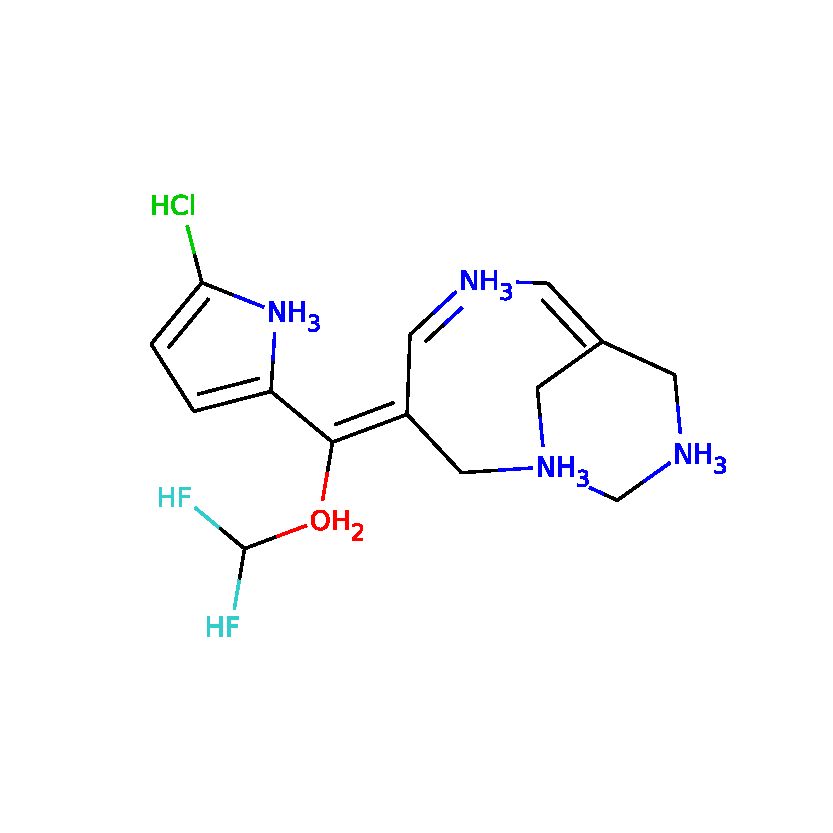
\includegraphics[width=0.22\textwidth]{figures/experiments_figures/molecule_samples/generated_molecule_796_v.pdf} & 
        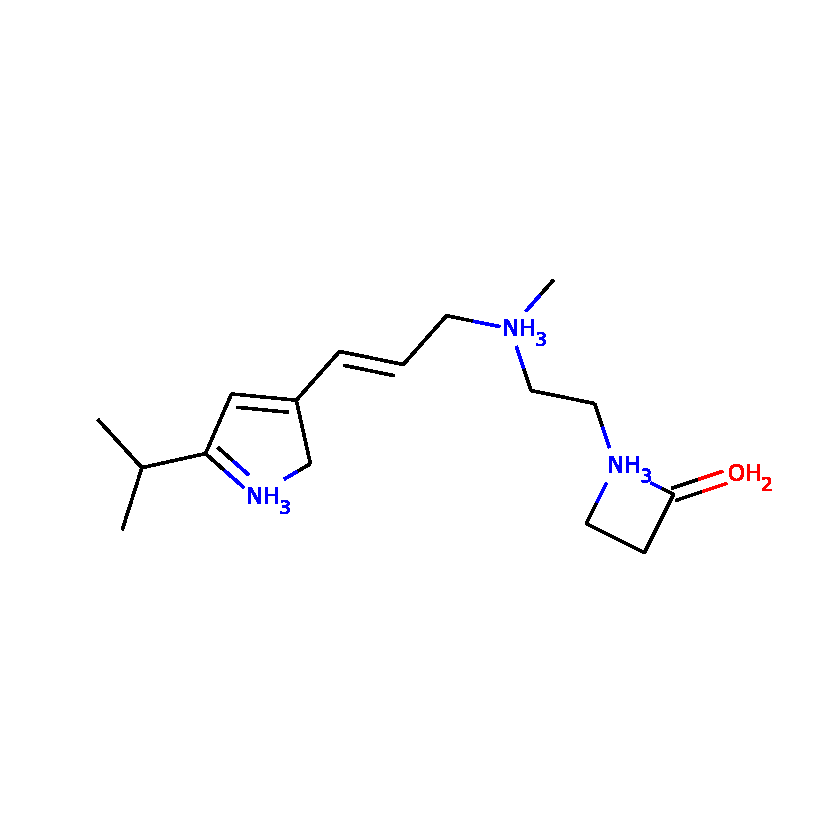
\includegraphics[width=0.22\textwidth]{figures/experiments_figures/molecule_samples/generated_molecule_1_v.pdf}  & 
        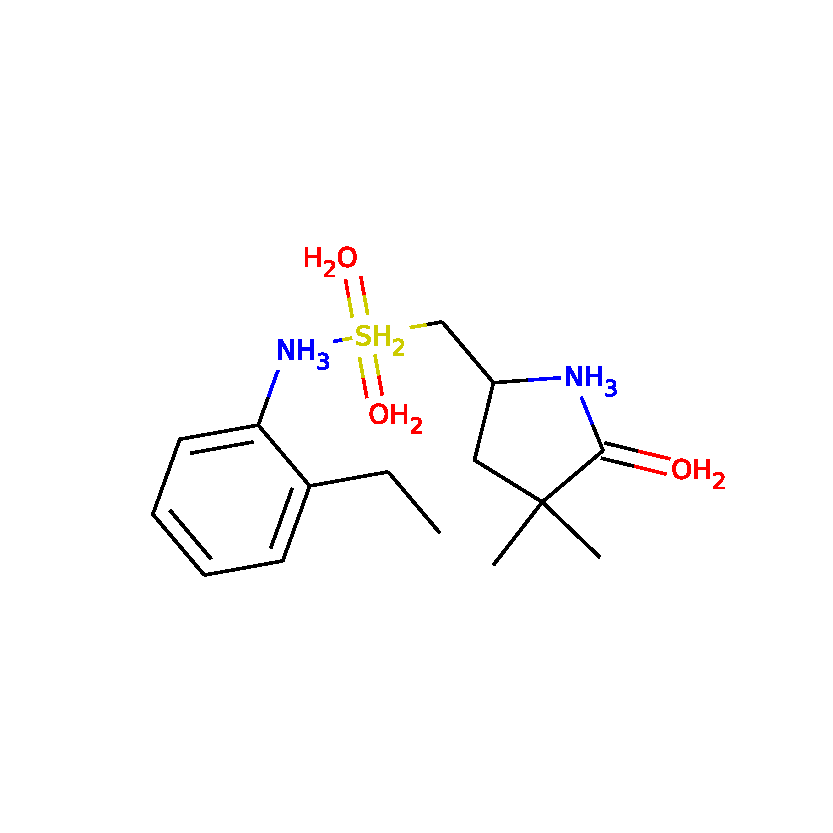
\includegraphics[width=0.22\textwidth]{figures/experiments_figures/molecule_samples/generated_molecule_6_v.pdf}  & 
        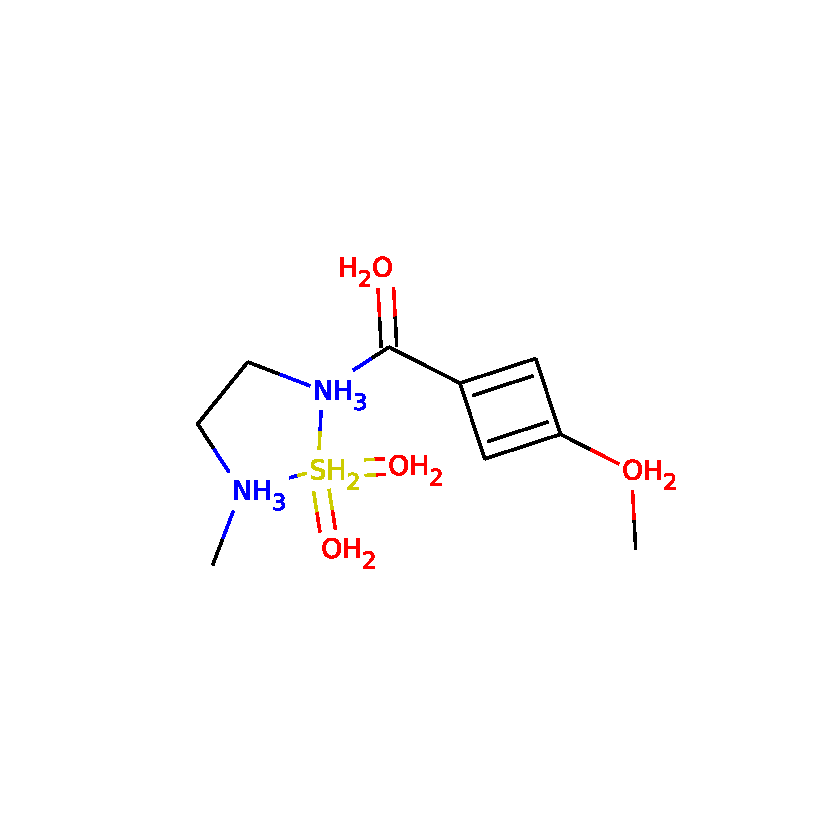
\includegraphics[width=0.22\textwidth]{figures/experiments_figures/molecule_samples/generated_molecule_8_v.pdf} \\ 
        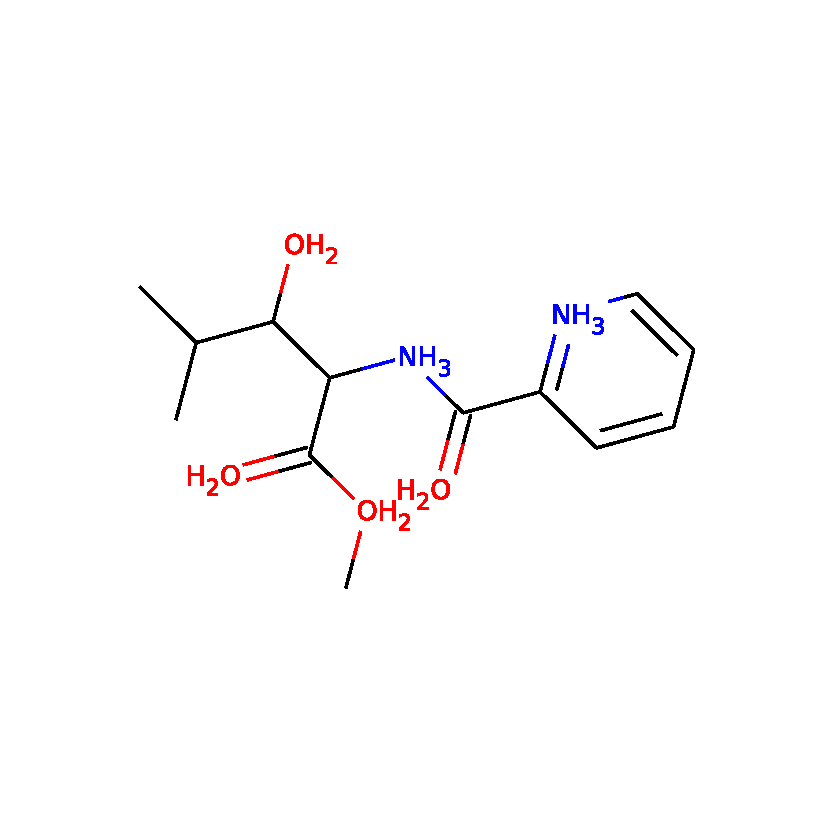
\includegraphics[width=0.22\textwidth]{figures/experiments_figures/molecule_samples/generated_molecule_10_v.pdf} & 
        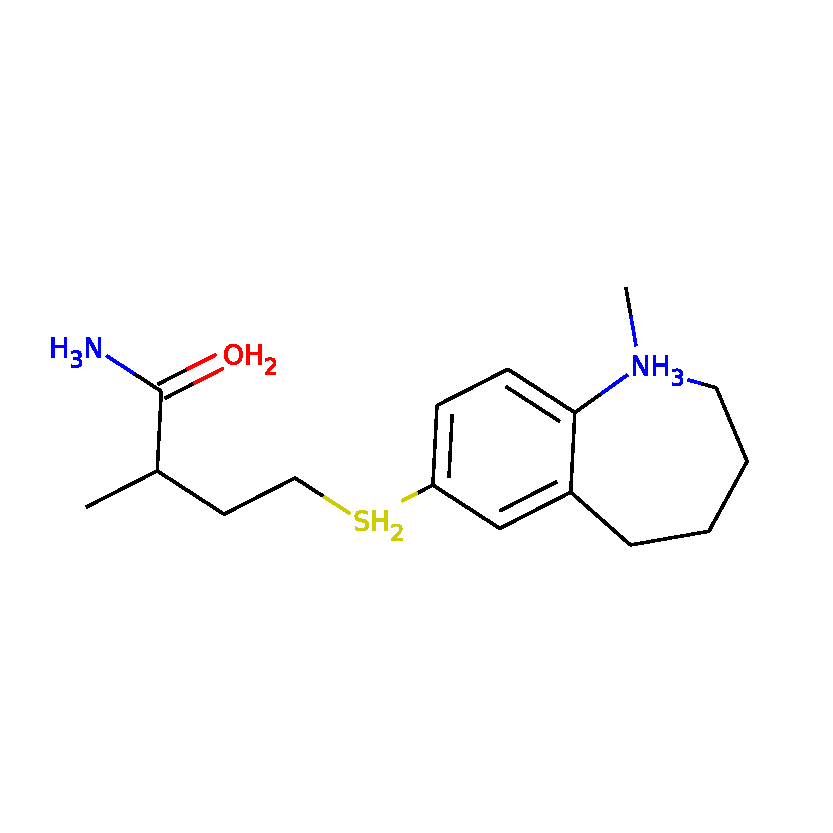
\includegraphics[width=0.22\textwidth]{figures/experiments_figures/molecule_samples/generated_molecule_13_v.pdf} &
        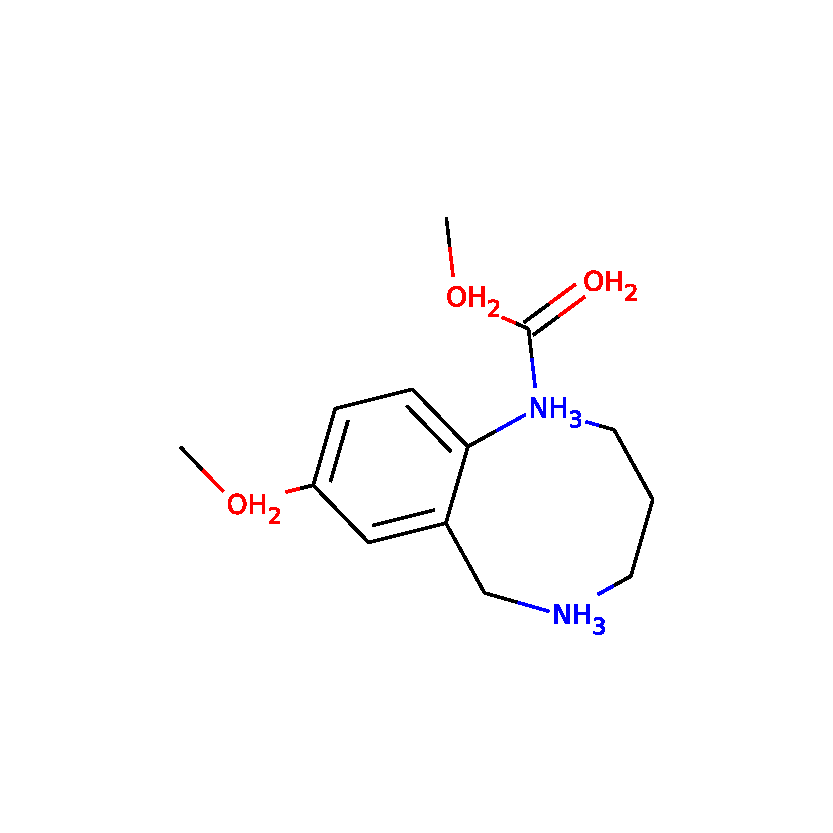
\includegraphics[width=0.22\textwidth]{figures/experiments_figures/molecule_samples/generated_molecule_16_v.pdf} &
        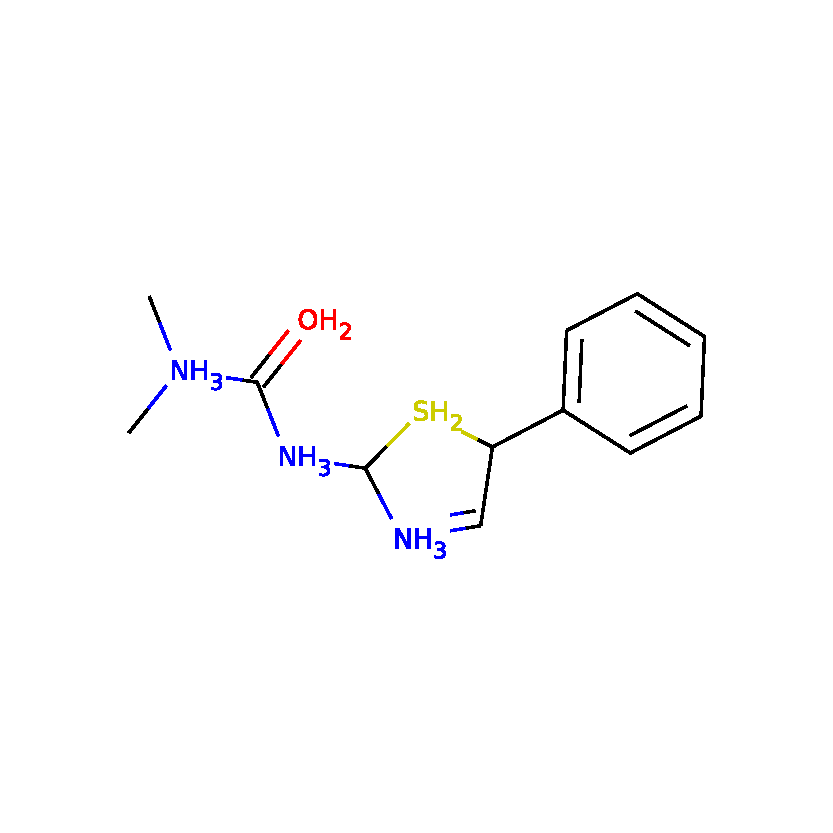
\includegraphics[width=0.22\textwidth]{figures/experiments_figures/molecule_samples/generated_molecule_19_v.pdf} \\
        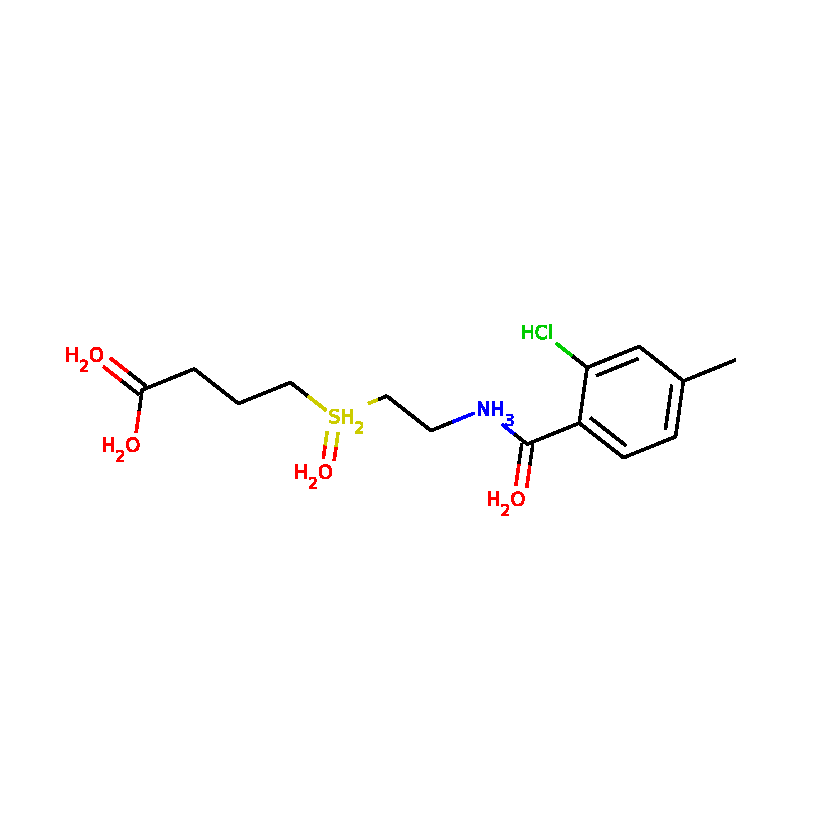
\includegraphics[width=0.22\textwidth]{figures/experiments_figures/molecule_samples/generated_molecule_120_v.pdf} & 
        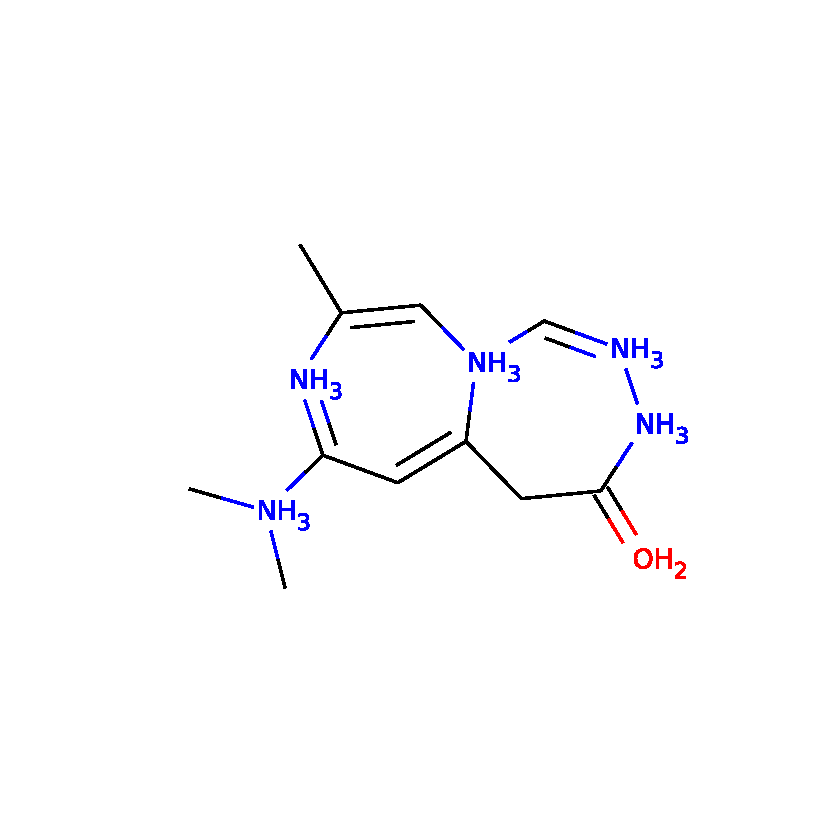
\includegraphics[width=0.22\textwidth]{figures/experiments_figures/molecule_samples/generated_molecule_22_v.pdf} &
        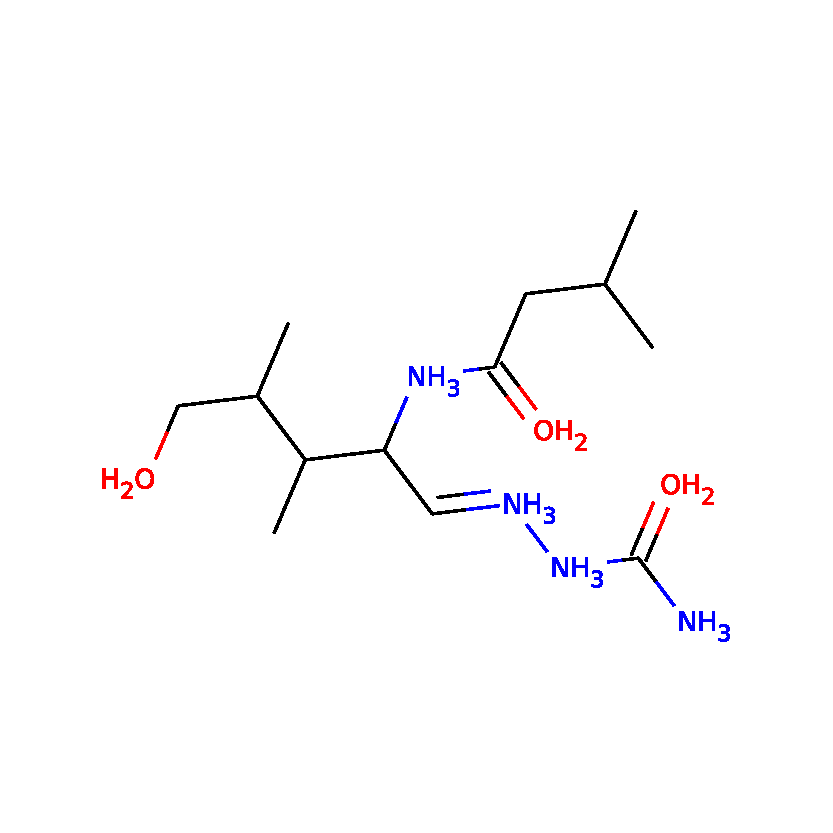
\includegraphics[width=0.22\textwidth]{figures/experiments_figures/molecule_samples/generated_molecule_23_v.pdf} &
        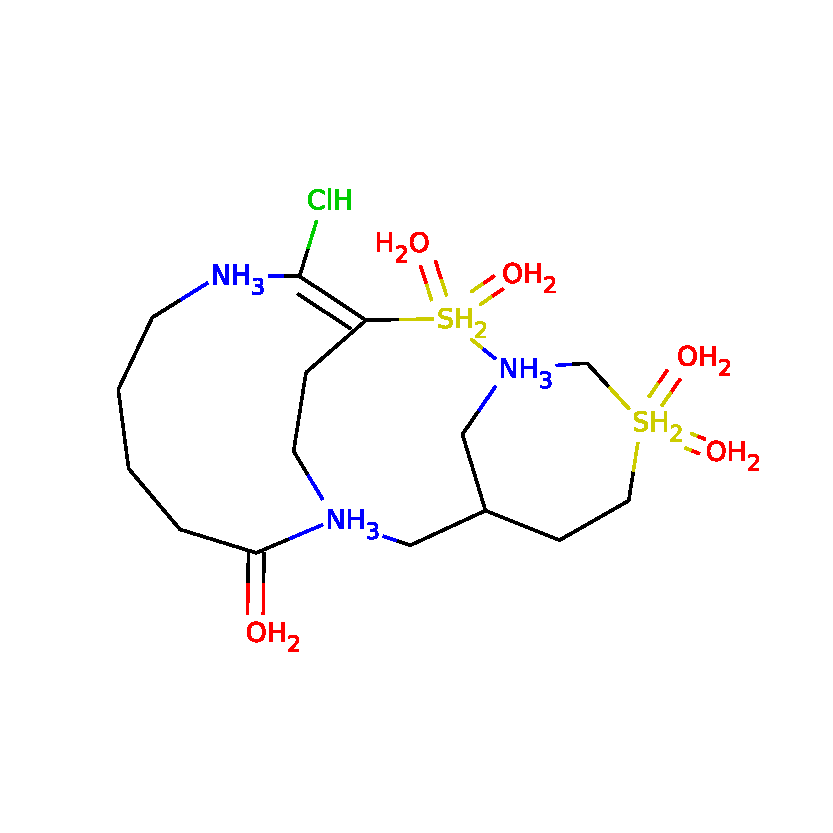
\includegraphics[width=0.22\textwidth]{figures/experiments_figures/molecule_samples/generated_molecule_269_v.pdf}
        \\
    \end{tabular}
    \caption[Samples of molecule graphs from GraphCNF]{Visualization of molecules generated by GraphCNF which has been trained on the Zinc250k \cite{Zinc250k} dataset. Nodes with black connections and no description represent carbon atoms. All of the presented molecules are valid. Best viewed in color and digitally for large molecules.}
    \label{fig:appendix_molecule_generation}
\end{figure}

\subsection{Language modeling}
\label{sec:experiments_language_modeling}

\paragraph{Task} Finally, we test Categorical Normalizing Flows on the task of language modeling. 
The goal of language modeling is to capture grammar and semantic rules of language from large text corpora, and has gained increasingly interest since the recent developments and capabilities of large language models \cite{BERT, GPT2, GPT3}.
Meanwhile, latent-based language models are mostly based on variational autoencoders and suffer in particular from posterior collapse, as decoders like autoregressive models tend to ignore the latent space.
Normalizing flows could potentially offer a new, more stable approach, as they do not rely on strong decoders and work with exact likelihood estimates. 


\paragraph{Datasets} We experiment with two popular character-level datasets, Penn Treebank \cite{PennTreeBank} and text8 \cite{text8}. 
The Penn Treebank consists of 5M characters and has a vocabulary size of $K=51$ characters.
We follow the setup of \citet{SemiDiscreteNFSequence} and split the dataset into sentences of a maximum length of 288. 
Text8 contains about 100M characters and has a vocabulary size of $K=27$. 
We again follow the preprocessing of \citet{mikolov2012subword} and train the models on an input sequence length of 256.
In addition to character-level experiments, we test our model on a word-level language modeling dataset, Wikitext103 \cite{Wikitext}, with a vocabulary size of $K=10,000$. 
Discrete Normalizing Flows are not able to handle such a high number of classes due to its approximations \cite{TranDiscreteFlows}, while Categorical Normalizing Flows can handle such vocabularies. 
Similar to text8, we train the models on a sequence length of 256 for Wikitext103.

\paragraph{Models} For the character-level datasets, we use an encoding dimensionality of 3 per token and increase it to 10 for the word-level experiment.
Each flow applies mixture coupling layers being autoregressive across time and latent dimensions. 
For the character-level experiments, we set the number of mixtures equals to the vocabulary size to verify our motivation on using the mixture coupling layers. 
In the case of the word-level experiment, we limit the number of mixtures to $64$.
We use the same LSTM \cite{LSTM} with hidden size 1024 for all flows and baselines. 

We compare Categorical Normalizing Flows against Latent Normalizing Flows by \citet{SemiDiscreteNFSequence} who reported results on the Penn Treebank dataset.
Their model uses a two-layer Bi-LSTM as encoder and decoder, and 5 flow layers for the prior.
To guarantee a fair comparison and pin down our comparison to the encoding strategy, we also implement a Latent Normalizing Flow with the setup of Categorical Normalizing Flows except the encoding and decoding, for which we use a two-layer Bi-LSTM predicting the mean and scale of logistic distributions.

\begin{table}[t]
	\caption[Results on language modeling]{Results on language modeling measured in bits per character and averaged across 3 seeds (standard deviation shown as $\pm...$). The reconstruction error, also in bits per character, is shown in brackets. Results by \citet{SemiDiscreteNFSequence} did not report a standard deviation.
	}
	\label{tab:result_table_token_level}
	\centering
	\setlength\tabcolsep{4mm}
	\begin{tabular}{lccc}
		\toprule
		\textbf{Model} & \textbf{Penn Treebank} & \textbf{text8} & \textbf{Wikitext103} \\
		\midrule
		LSTM baseline & $1.28$ \footnotesize{$\pm0.01$} & $1.44$ \footnotesize{$\pm0.01$} & $4.81$ \footnotesize{$\pm0.05$}\\[4pt]
		Latent NF & & & \\
		- \citet{SemiDiscreteNFSequence} & $1.42$ \footnotesize{(0.10)} & $-$ & $-$ \\
		- 1 layer & $1.40$ \footnotesize{$\pm0.02$} \footnotesize{(0.04)} & $1.61$ \footnotesize{$\pm0.01$} \footnotesize{(0.03)} & $7.05$ \footnotesize{$\pm0.31$} \footnotesize{(1.09)}\\
		\midrule
		Categorical NF - 1 layer & $1.27$ \footnotesize{$\pm0.01$} \footnotesize{(0.00)} & $1.45$ \footnotesize{$\pm0.01$} \footnotesize{(0.00)} & $5.43$ \footnotesize{$\pm0.09$} \footnotesize{(0.32)}\\
		\bottomrule
	\end{tabular}
\end{table}

\paragraph{Results} The results in Table~\ref{tab:result_table_token_level} show that Categorical Normalizing Flows with a single layer are performing on par with their non-latent autoregressive counterparts. 
The reconstruction loss of the discrete tokens from continuous space, i.e. the average negative log-likelihood of the decoder, is lower than $1e$-$3$bpd showing that the posterior is almost deterministic. 
Furthermore, when comparing to \citet{SemiDiscreteNFSequence}, we see a significant improvement while using only 1 instead of 5 flows and a much simpler encoding.
Our re-implementation 
This underlines the importance of using a factorized posterior and removing any interactions between variables from the decoder. 
One notable difference between our setup of Latent NF and \citet{SemiDiscreteNFSequence} is the lower reconstruction error despite the prior being considerably smaller in number of parameters and depth. 
As the only other major difference is the type of coupling layer (\citet{SemiDiscreteNFSequence} use non-linear squared flows), we can conclude that mixture coupling layers promote the shift of likelihood optimization towards the prior, and push the decoder to being deterministic.

For word-level language modeling, a single mixture coupling layer is not flexible enough to learn all possible sequences.
Thus, we see a small gap between the LSTM baseline and Categorical Normalizing Flows, although the flow's flexibility could be improved by using more transformations/layers.
Nonetheless, this experiment shows that Categorical Normalizing Flows can generalize to large categorical distributions without being limited by gradient approximations or such.
In contrast, Latent Normalizing Flows achieve a considerably worse performance which is also attributed to training difficulties. 
Since decoding $10,000$ categories from a latent space is a challenging task in itself, we experienced instabilities when balancing the reconstruction error of the decoder with the prior likelihood.
These instabilities are also because the decoder, encoder and prior all work on the same latent space but changes in the encoding need to be propagated to the decoder and prior by consecutive gradient updates (i.e. decoder and prior run a step behind the encoder).
Categorical Normalizing Flows, on the other hand, did not show to have those issues as the decoder is independently applied across categorical variables, and therefore much simpler than in Latent Normalizing Flows.

\subsection{Discussion}
\label{sec:experiments_discussion}

The experiments on sets, graphs, and language modeling show that Categorical Normalizing Flows are widely applicable and can model categorical distributions precisely.
In the following section, we will discuss the important aspects of Categorical Normalizing in more detail.
In particular, we take another look at the encoding distributions and elaborate on the reasons why the mixture model is sufficient.
We also visualize the latent space of trained flows to gain further insights into the modeling capability of Categorical Normalizing Flows.
We conclude this section by discussing the differences to Discrete Normalizing Flows under the consideration of the obtained experimental results.

\subsubsection{Encoding distributions} 

Across all the tasks that we experimented on, the simple mixture model encoding has shown to work well with Categorical Normalizing Flows while being the most efficient at the same time.
Despite the additional flexibility, we experienced that the linear flow and variational encoding method mainly relied on a logistic mixture model as well.
This finding might seem counter-intuitive at first as several works have reported a significant gain by applying strong encoding distribution in variational dequantization for the task of image modeling \cite{Flow++, EmielDequantization, VFlow}. 

Besides the natural integration of logistics in our flow architecture which presumably leads to the favoring of a logistic encoding, there are two differences between categorical encoding and dequantization that are potentially crucial for the variational framework. 
Firstly, images are quantized, continuous signals that inherently contain noise from several sources \cite{NoiseModelsImages}. 
This noise can be both independent across pixels (e.g. white noise) or correlated with close-by pixels.
Variational dequantization can model this noise by a flexible dequantization distribution which needs to be complex enough to capture the noise's true mean and variance. 
In categorical distributions, however, we do not have such noise signals as categories are naturally discrete.  

Secondly, in dequantization, the encoding volumes of discrete values have sharp edges, i.e. the probability density function has a sudden change to zero.
As discussed by \citet{Flow++}, such volumes are more challenging to model for a normalizing flow as it requires several additional transformations.
Allowing the flow to change the encoding distribution in the first place simplifies the modeling objective.
Meanwhile, in Categorical Normalizing Flows, we do not have this issue as the volumes per category are separated with regions of low probability density between them, and usually do not contain sharp edges.
Thus, based on these two aspects, we argue that variational encoding does not (significantly) improve the modeling capabilities of Categorical Normalizing Flows, although it is important in the image domain.

The encoding distributions of Categorical Normalizing Flows all rely on the idea of having a factorized decoder across categorical variables.
This not only provides the encoding to be efficient during sampling, but also allows for an exact likelihood estimate in the case of a mixture model or linear encoding.
Latent Normalizing Flows, on the other hand, introduce interactions among variables in the decoder, and thus, models a lower bound. 
In general, we found Latent Normalizing Flows only to work well when we were able to train the decoder to be close to deterministic.
This was the case for the set modeling experiments and the character language modeling, with applying an appropriate loss scheduling, but not for the word-level experiments due to the large number of categories.
Still, in all experiments we experienced Latent NFs to be instable, in particular in the beginning of the training when the decoder propagates high gradients back to the encoder. 
This causes the encoding distribution to change abruptly, and the prior has to adapt to these changes within the next iterations. 
However, this can again lead to a high loss when the transformations in the prior do not fit to the new encoding, and thus map them to points of low likelihood.
Thus, we see a loss peak across couple of iterations until the model balances itself out again, or diverges.
Such situations were encouraged by having rare categories in the dataset, as in the Penn Treebank and Wikitext103.  

Compared to Latent Normalizing Flows, Categorical Normalizing Flows offer two benefits.
Firstly, CNFs are more stable and simpler to train as no loss scheduling is required, and the likelihood remains an exact estimate.
Secondly, the encoding of CNFs is much more efficient than Latent NFs. 
Despite selecting suitable encoder and decoder architectures for the respective tasks, the additional complexity did not show to help in our experiments. 
Thus, we come to the conclusion that Categorical Normalizing Flows are more widely applicable, and Latent NFs might only the better choice if there exists a task-specific decoder that integrates pre-known knowledge about the data.

\subsubsection{Visualization of the latent space} 
\label{sec:experiments_discussion_latent_space}

To gain insights into the inner working of Categorical Normalizing Flows, we visualize the latent space at different stages of the flow.
We hope to see interactions among categories and understand how Categorical Normalizing Flows utilize continuous transformations to learn categorical distributions.
For visualization purposes, we limit the latent space dimensionality to 2 and accumulate the samples across categorical variables. 
We show the mapping of the mixture model to a single logistic by color-coding the modes of each category differently.
The samples in the forward direction are gathered from about 1k categorical data points, each sampled 8 times from the encoding distribution.
For inverting the flow, we sampled 8k times from the base distribution.
For reproducibility, the exact details of the visualization are summarized in Appendix~\ref{sec:appendix_latent_space_visualization}.

\begin{figure}[t!]
    \centering
    \begin{subfigure}{\textwidth}
        \centering
        \begin{tabular}{cccc}
            \textit{Encoding distribution} &
            \textit{Flow layer 4} & 
            \textit{Flow layer 6} & 
            \textit{Base distribution} \\
            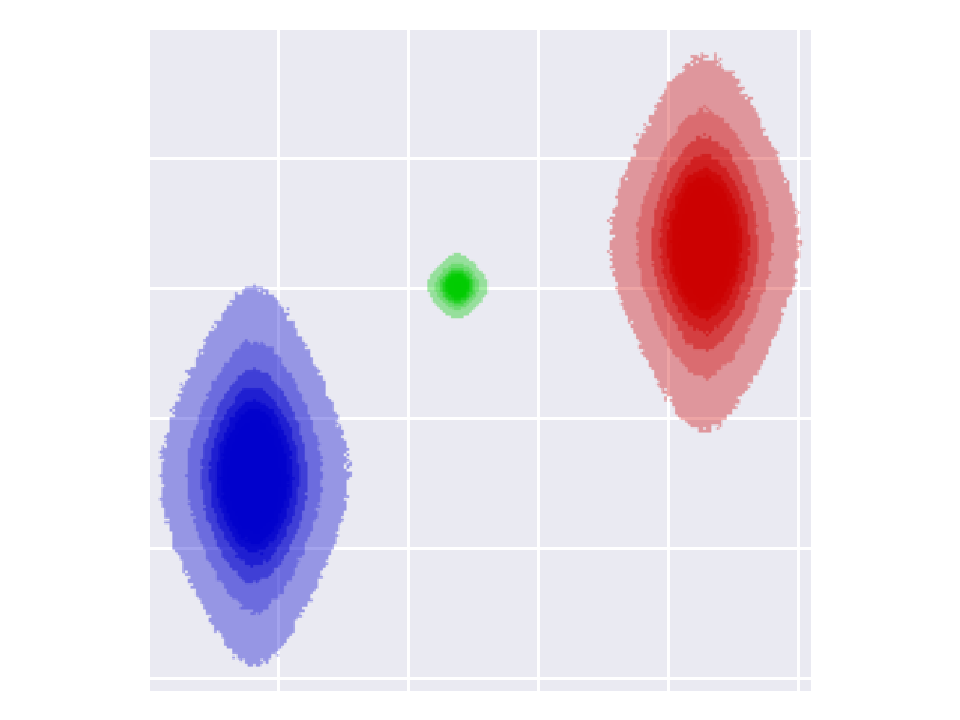
\includegraphics[width=0.225\textwidth]{figures/experiments_figures/latent_space/graph_coloring/layer_forward_01.pdf} & 
            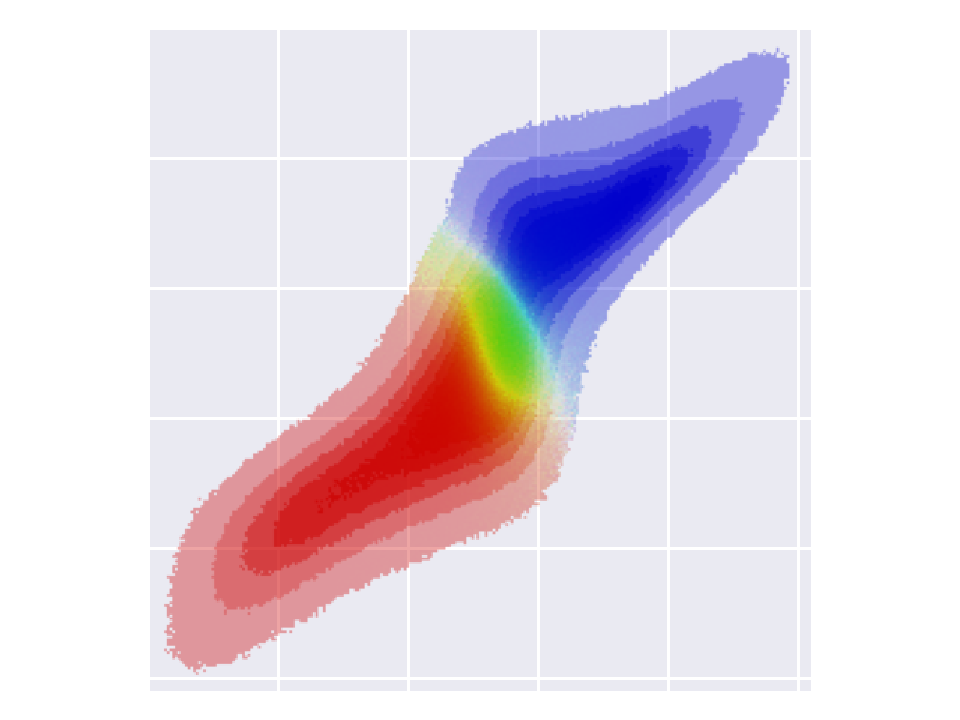
\includegraphics[width=0.225\textwidth]{figures/experiments_figures/latent_space/graph_coloring/layer_forward_13.pdf}  & 
            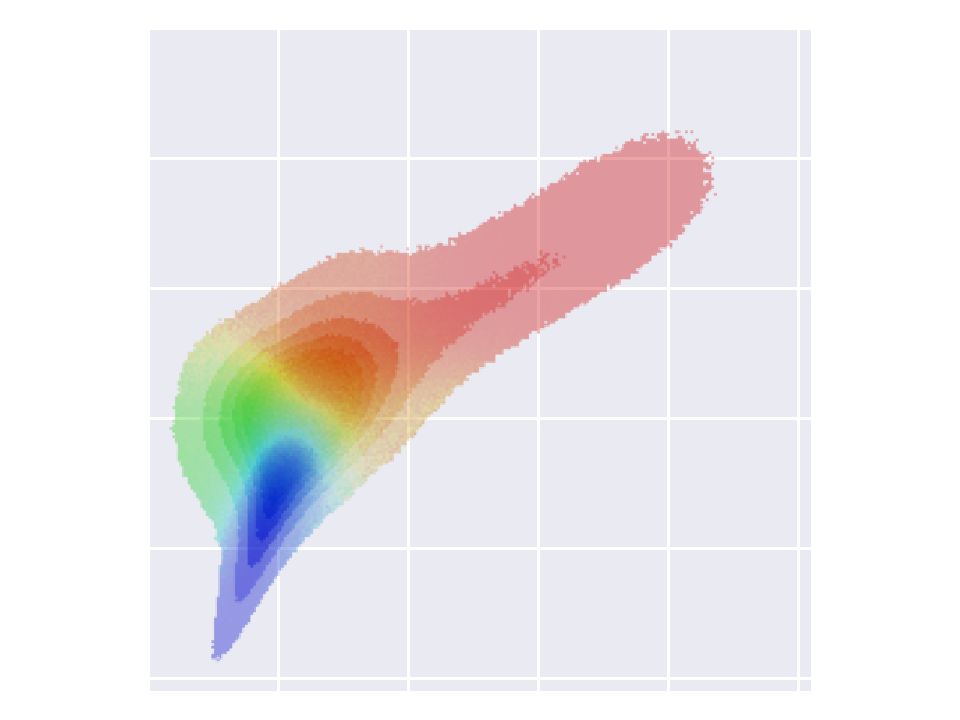
\includegraphics[width=0.225\textwidth]{figures/experiments_figures/latent_space/graph_coloring/layer_forward_19.pdf}  & 
            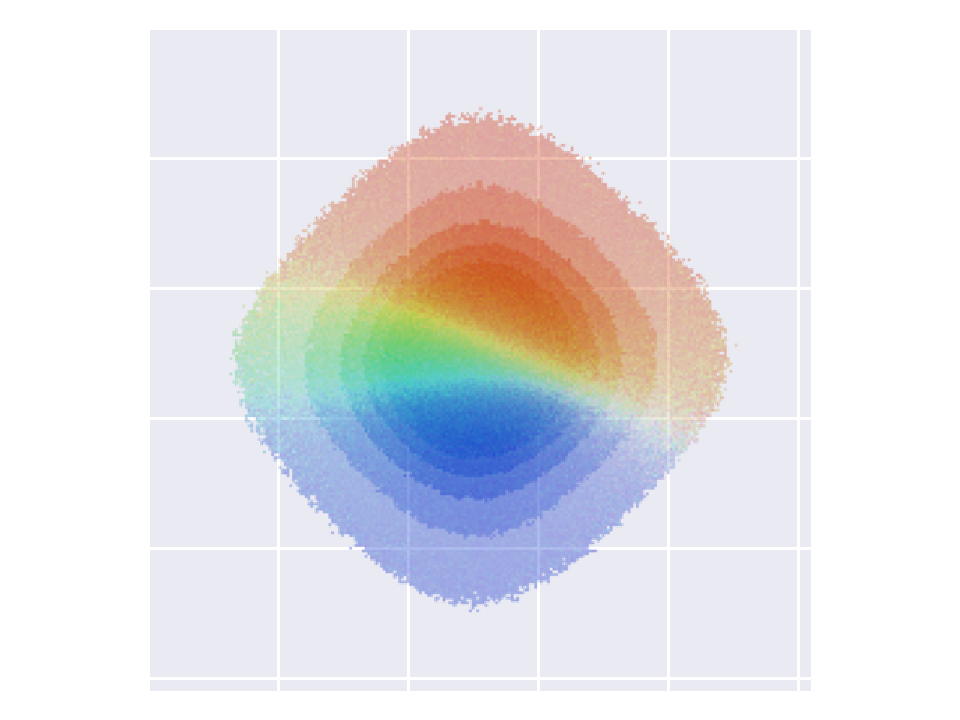
\includegraphics[width=0.225\textwidth]{figures/experiments_figures/latent_space/graph_coloring/layer_forward_25.pdf}
            \\
        \end{tabular}
        \caption{Forward sampling\\[0.5cm] }
    \end{subfigure}
    \begin{subfigure}{\textwidth}
        \centering
        \begin{tabular}{cccc}
            \textit{Encoding distribution} &
            \textit{Flow layer 4} & 
            \textit{Flow layer 6} & 
            \textit{Base distribution} \\
            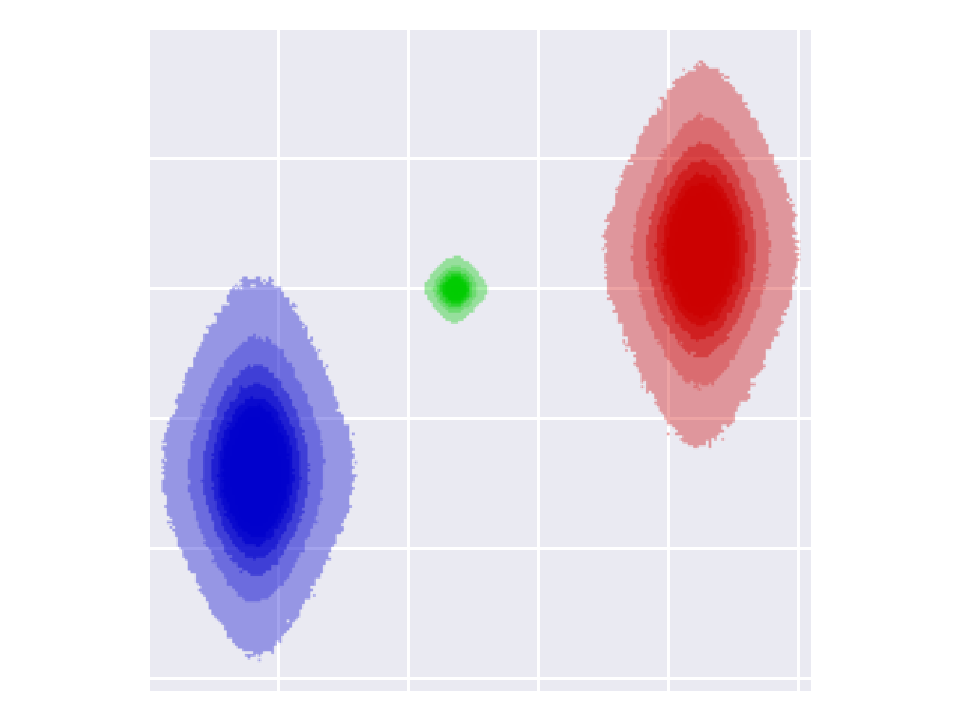
\includegraphics[width=0.225\textwidth]{figures/experiments_figures/latent_space/graph_coloring/layer_reverse_26.pdf} & 
            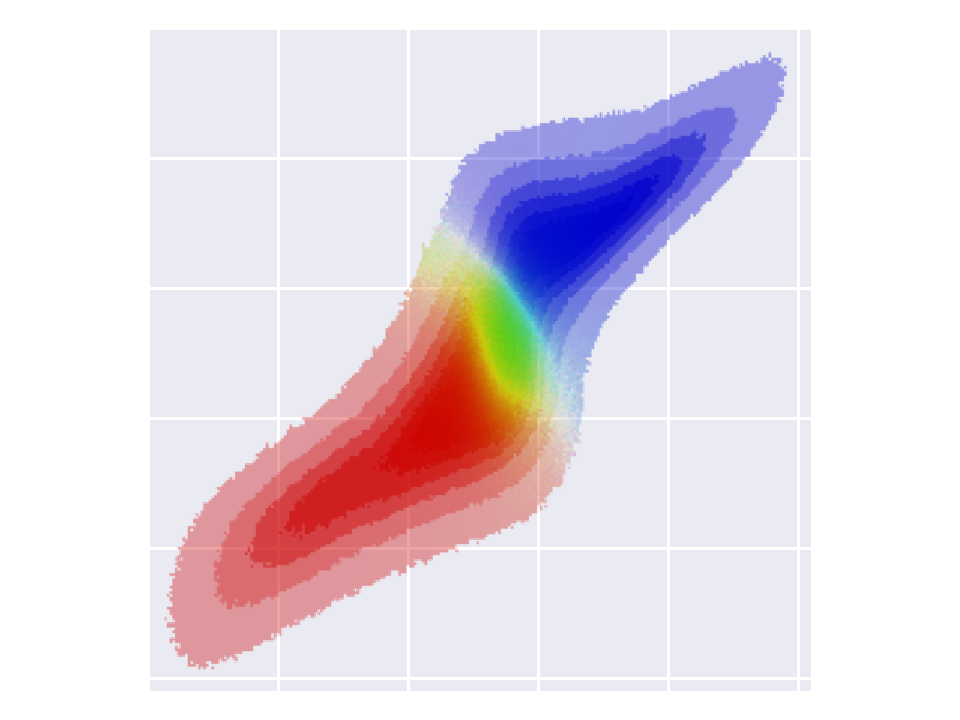
\includegraphics[width=0.225\textwidth]{figures/experiments_figures/latent_space/graph_coloring/layer_reverse_14.pdf}  & 
            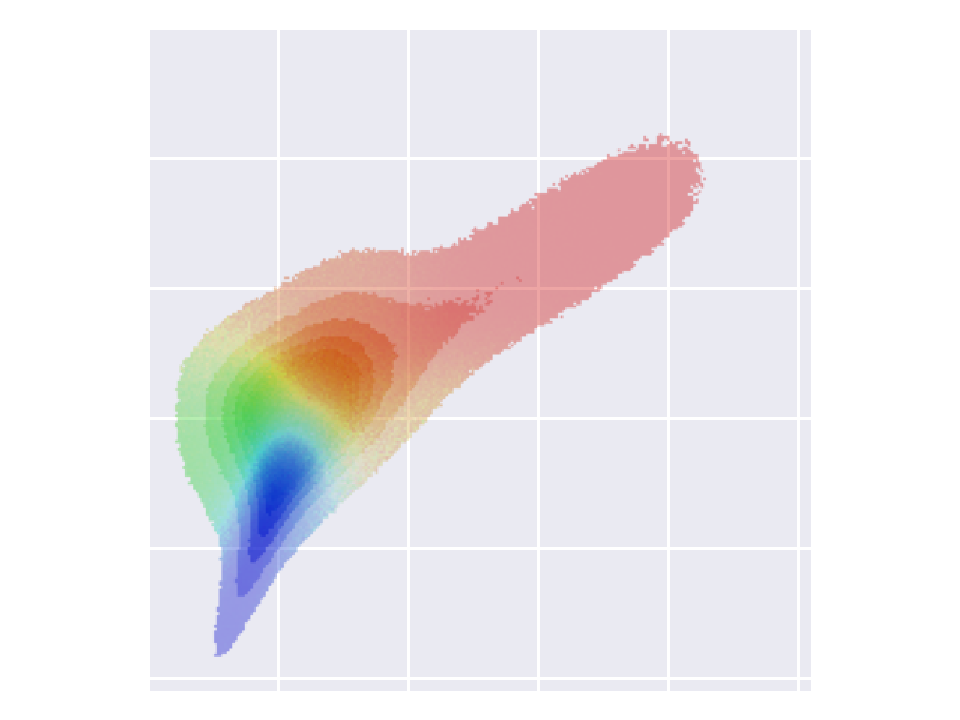
\includegraphics[width=0.225\textwidth]{figures/experiments_figures/latent_space/graph_coloring/layer_reverse_08.pdf}  & 
            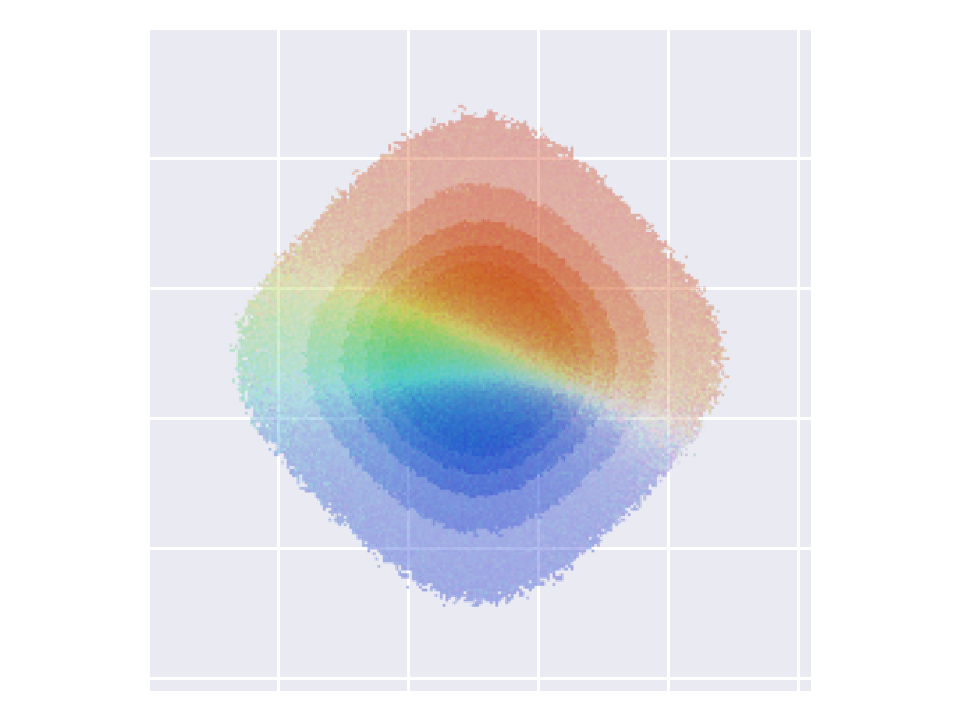
\includegraphics[width=0.225\textwidth]{figures/experiments_figures/latent_space/graph_coloring/layer_reverse_02.pdf}
            \\
        \end{tabular}
        \caption{Reverse sampling\\[0.2cm]}
        \label{fig:experiments_discussion_latent_space_graph_coloring_reverse}
    \end{subfigure}
    \caption[Latent space of graph coloring flow]{Visualization of the latent space in a 8-layer flow trained on graph coloring with 3 categories (shown in red, blue and green; best viewed in color and digital). The density of each category is colored differently and normalized independently. Overlapping distributions are shown by averaging the RGB colors weighted by their probability density. The left most figure shows the learned mixture encoding distribution $q(\bm{z}|\bm{x})$, the center figures show the latent spaces after corresponding coupling flow layers and right most shows the modeled base distribution (logistic). The latent space is scaled to fit into the figure size for each visualization independently. Subfigure (a) shows the probability densities in forward mode, i.e. pushing dataset examples through the flow, and (b) during generation, i.e. when sampling from the base distribution and reversing the flows.
    A larger visualization of all flow layers can be found in Appendix~\ref{sec:appendix_latent_space_visualization}.}
    \label{fig:experiments_discussion_latent_space_graph_coloring}
\end{figure}

Figure~\ref{fig:experiments_discussion_latent_space_graph_coloring} shows the latent space of a GraphCNF model on the task of graph coloring.
The model is trained on the small dataset as a latent dimensionality of 2 has shown to work well there.
The encoding distribution is, as expected, a mixture of three logistic distributions, each with a different mean and scale.
Interestingly, the green color has a significantly smaller scale than the other two, but this pattern is not constant across seeds. 
The layers in between show that the categories are stepwise merged, depending on the specific input/node in a graph.
While in layer 4 we have small areas where multiple categories occur (the yellow, cyan, and purple areas), most parts can be clearly associated with one color.
In layer 6, the combined area is growing and takes on a significant part of the overall probability density.
Finally, the base distribution still seems to be split into three parts, one for each category.
However, when looking closely at the respective parts, we can see that the colors are not pure, meaning that there is also a considerable amount of samples from the other two categories in the parts.
For instance, the red part is \textit{sprinkled} with yellow and purple pixels (the exact location is possibly due to the variance in the visualization).
Hence, we can say that each part resembles a \textit{dominant} color, i.e. if possible the node will be colored respectively, but also supports different colors when necessary.

The latent space that is created when inverting the flows (Figure~\ref{fig:experiments_discussion_latent_space_graph_coloring_reverse}), i.e. during sampling, is almost exactly the same as in the forward direction. 
Minor differences can be spotted in flow layer 6 for the red density for instance, but those do not influence the samples in categorical space. 
Thus, we can validate that the encoding distribution does not constitute any difficulties to the flow and that the flow can accurately model the mixture input distribution.

\begin{figure}[t!]
    \centering
    \begin{subfigure}{\textwidth}
        \centering
        \begin{tabular}{cccc}
            \textit{Encoding distribution} &
            \textit{Flow layer 2} & 
            \textit{Flow layer 3} & 
            \textit{Base distribution} \\
            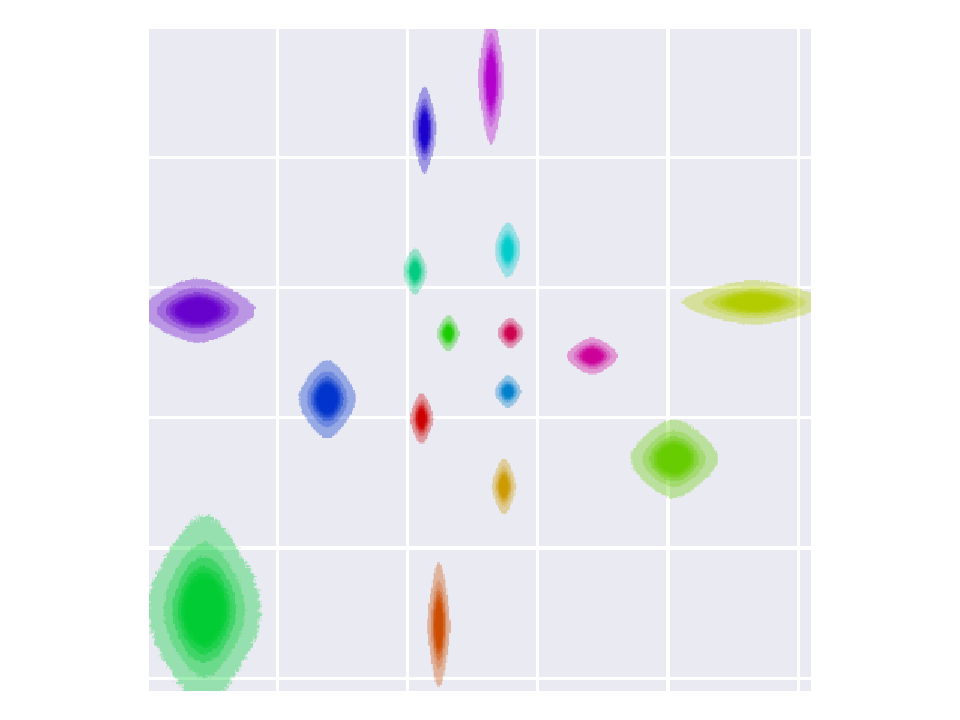
\includegraphics[width=0.225\textwidth]{figures/experiments_figures/latent_space/set_modeling/layer_forward_01.pdf} & 
            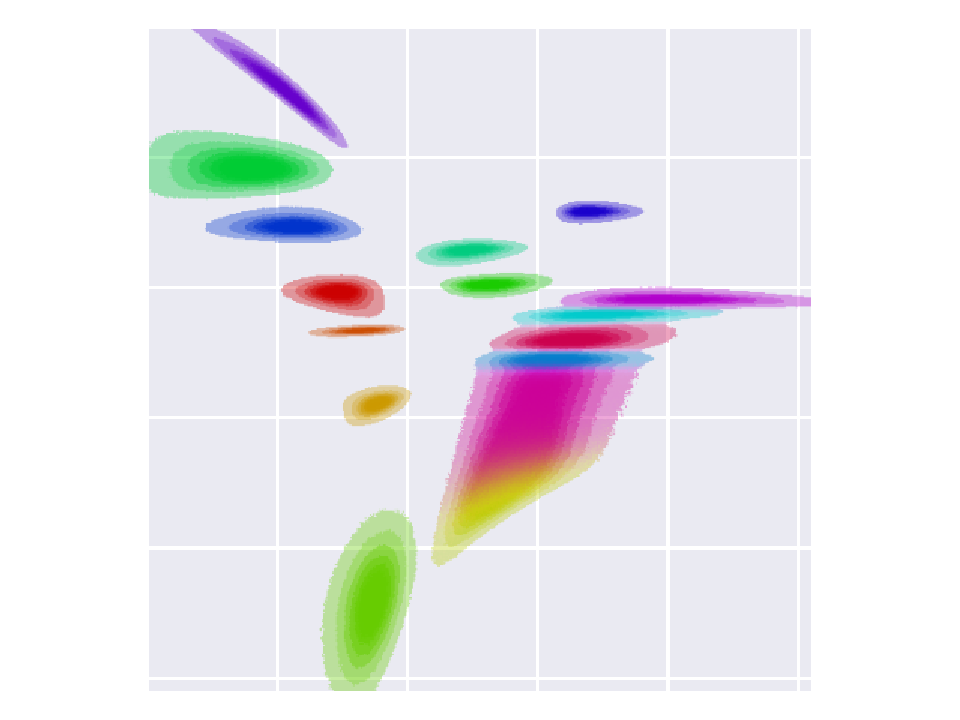
\includegraphics[width=0.225\textwidth]{figures/experiments_figures/latent_space/set_modeling/layer_forward_07.pdf}  & 
            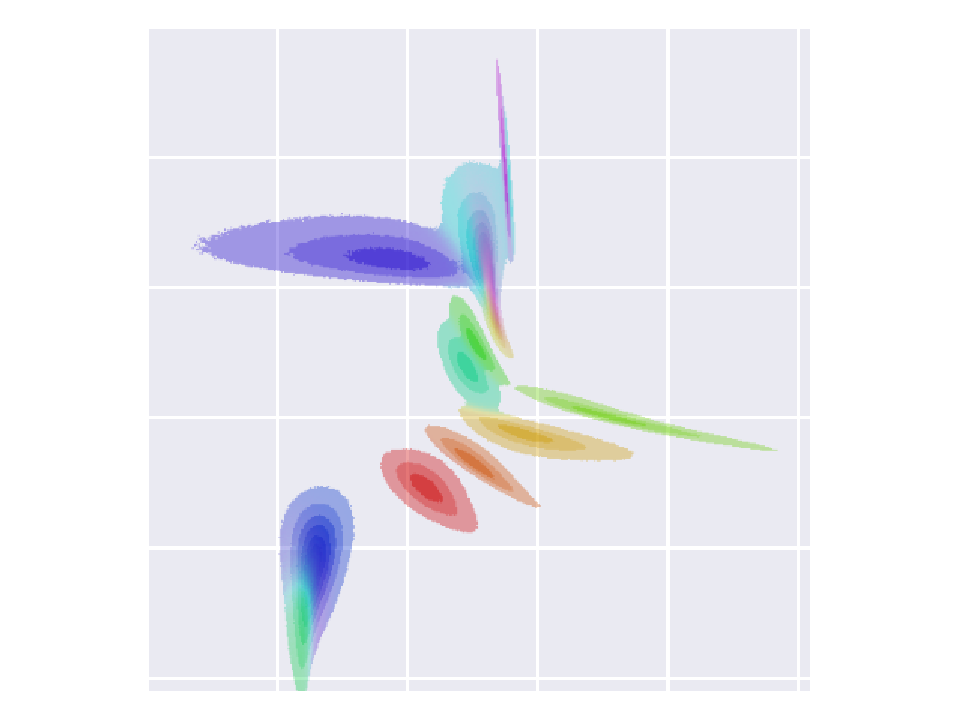
\includegraphics[width=0.225\textwidth]{figures/experiments_figures/latent_space/set_modeling/layer_forward_10.pdf}  & 
            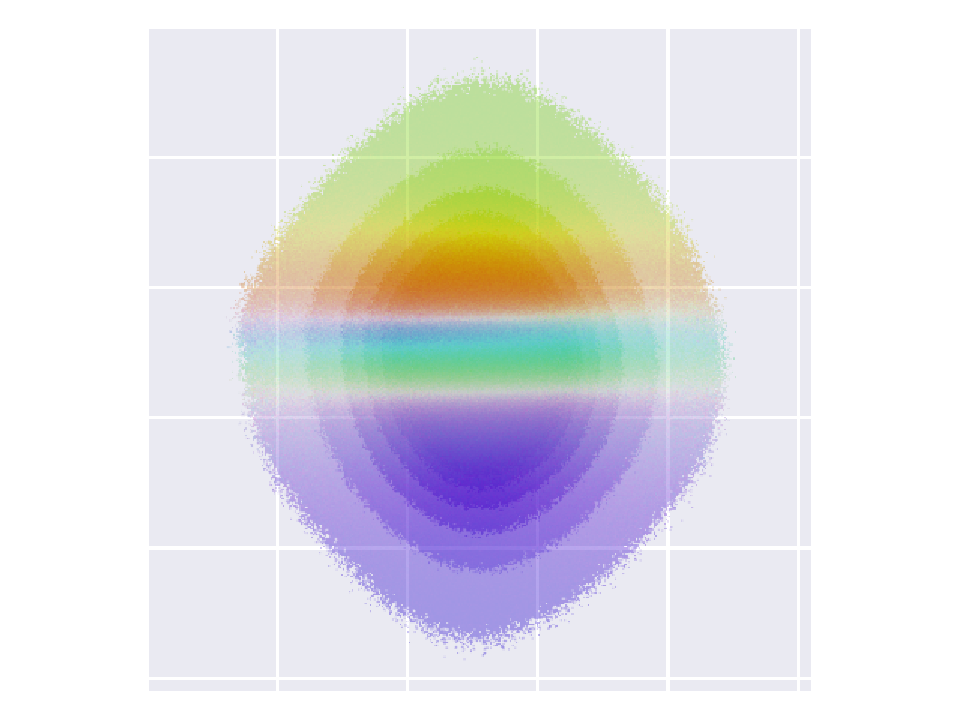
\includegraphics[width=0.225\textwidth]{figures/experiments_figures/latent_space/set_modeling/layer_forward_13.pdf}
            \\
            \multicolumn{4}{c}{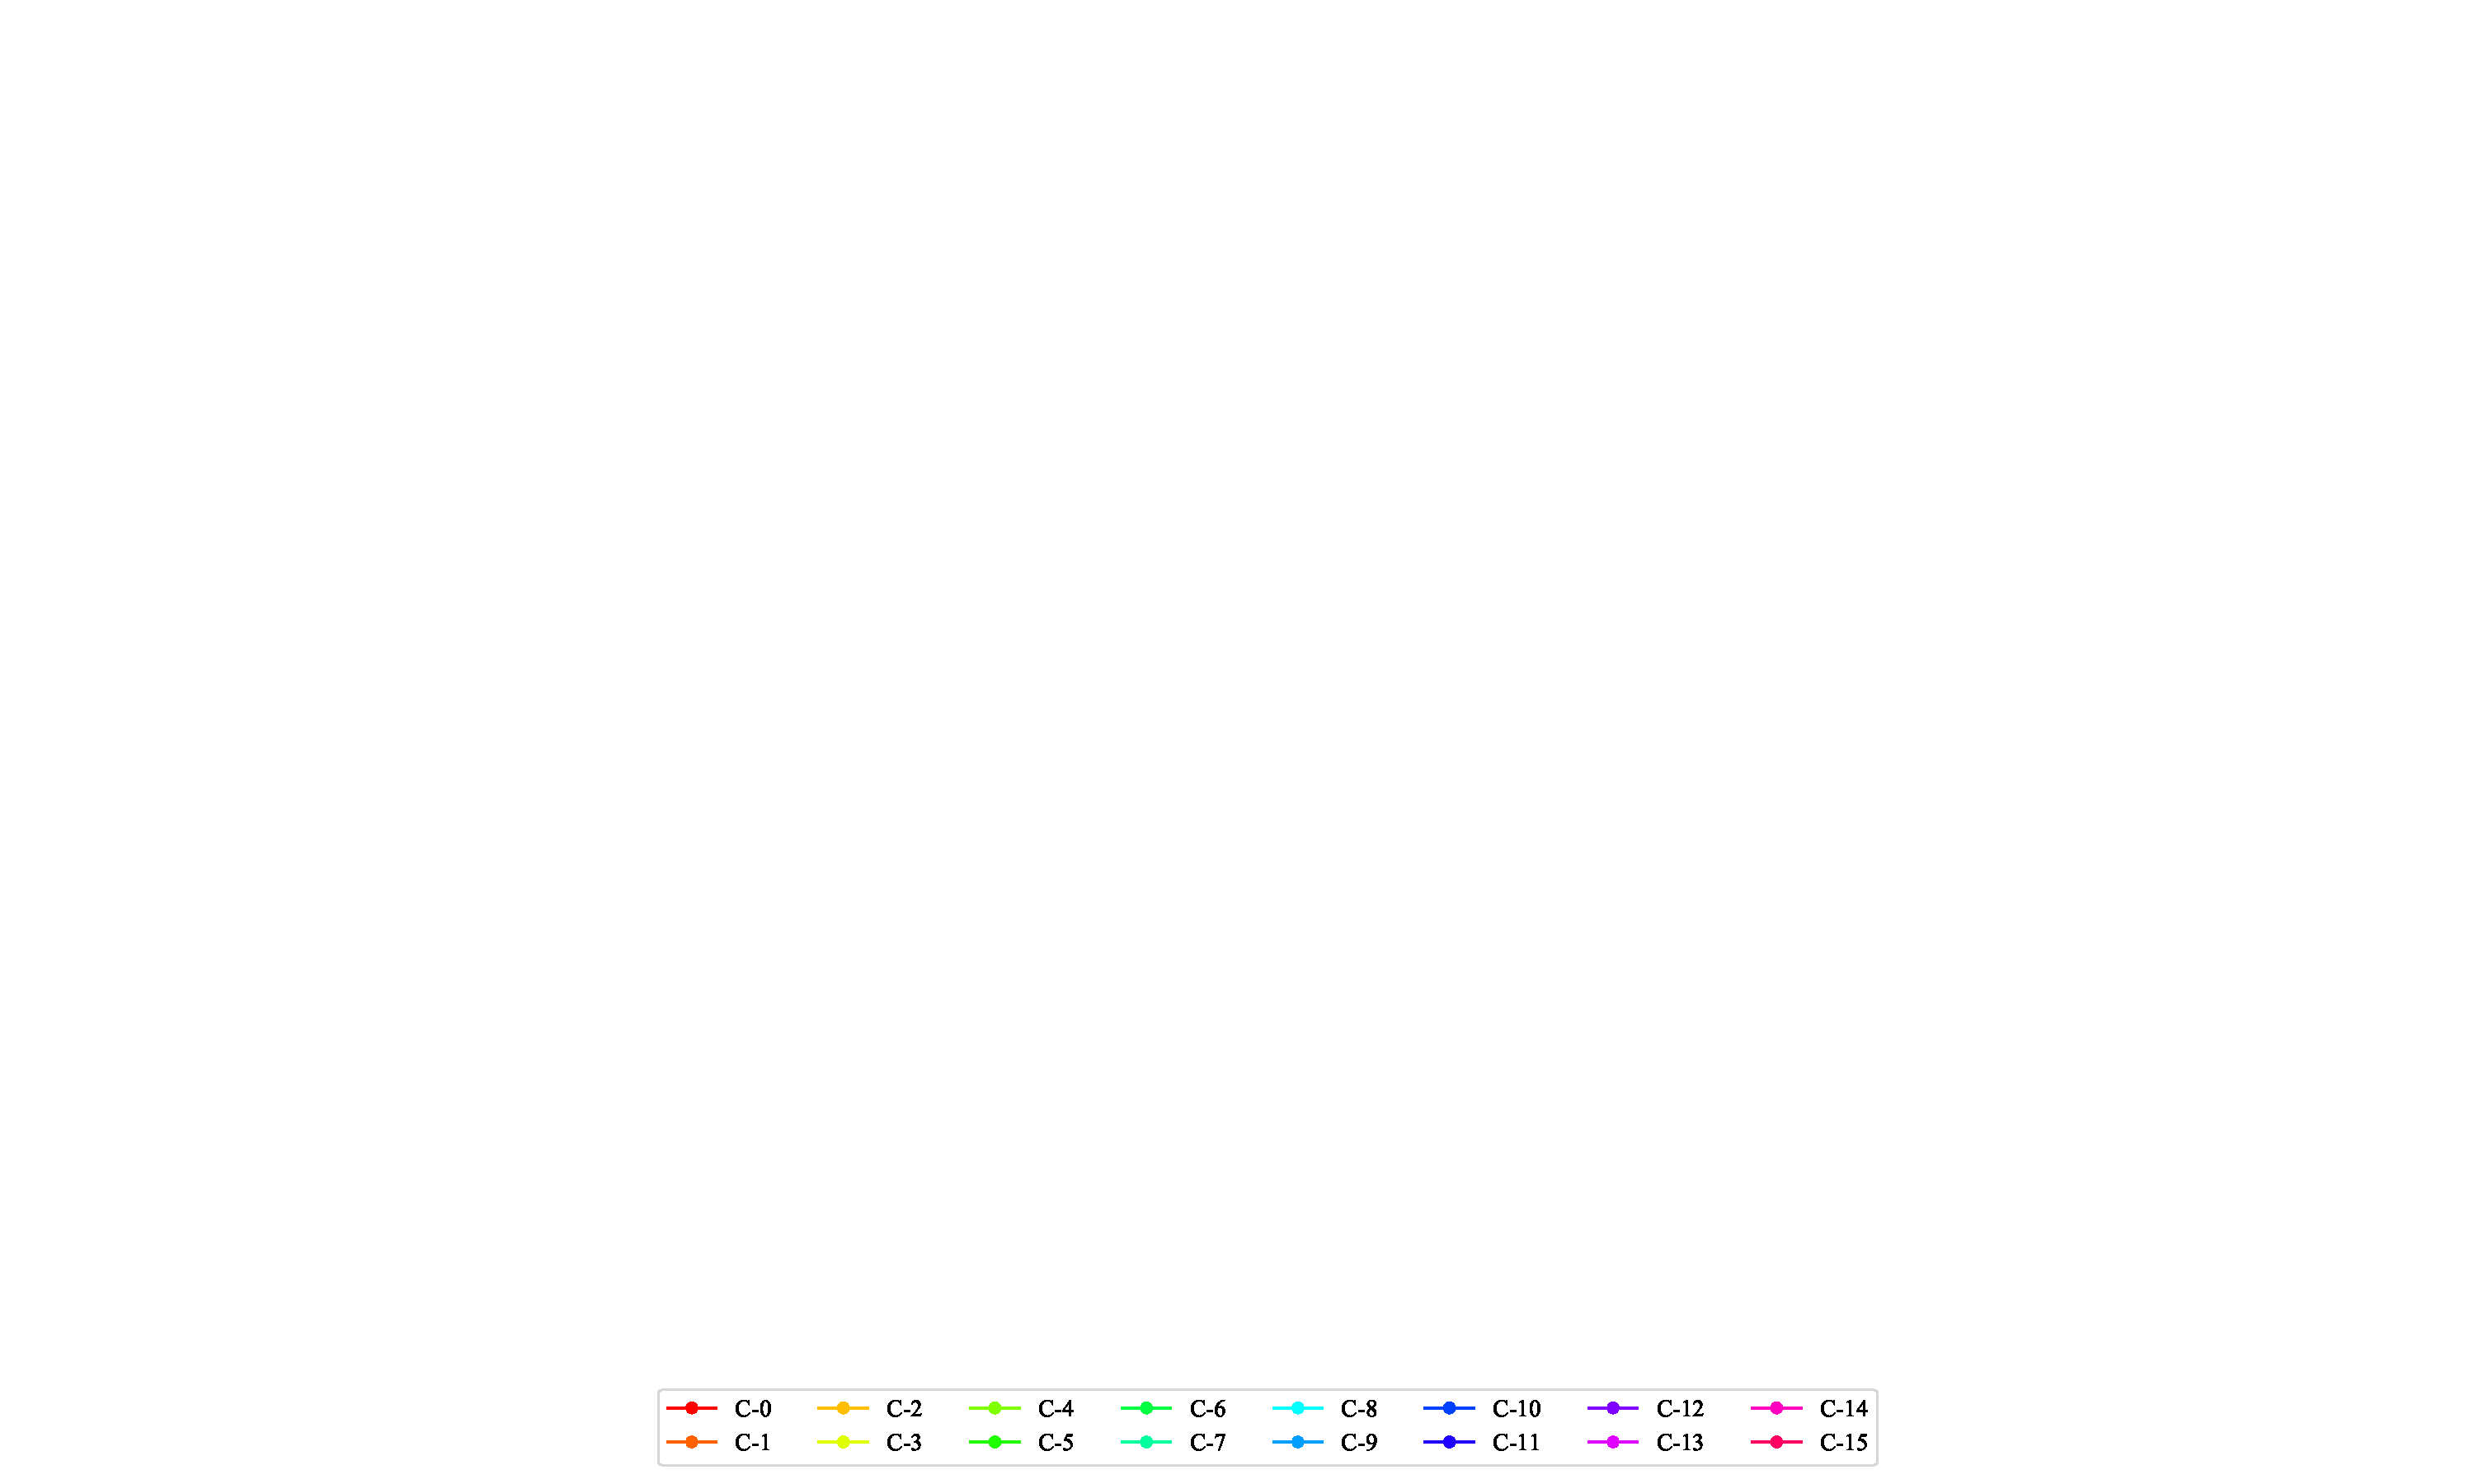
\includegraphics[width=0.95\textwidth]{figures/experiments_figures/latent_space/set_modeling/legend_visu.pdf}}\\
        \end{tabular}
        \caption{Forward sampling\\[0.5cm] }
    \end{subfigure}
    \begin{subfigure}{\textwidth}
        \centering
        \begin{tabular}{cccc}
            \textit{Encoding distribution} &
            \textit{Flow layer 2} & 
            \textit{Flow layer 3} & 
            \textit{Base distribution} \\
            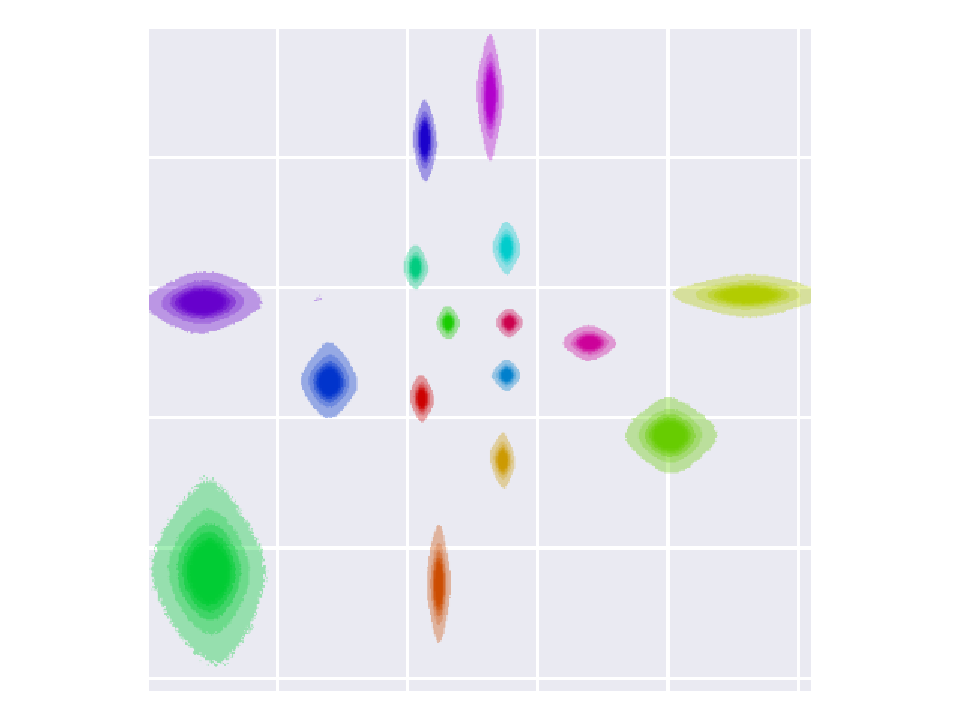
\includegraphics[width=0.225\textwidth]{figures/experiments_figures/latent_space/set_modeling/layer_reverse_13.pdf} & 
            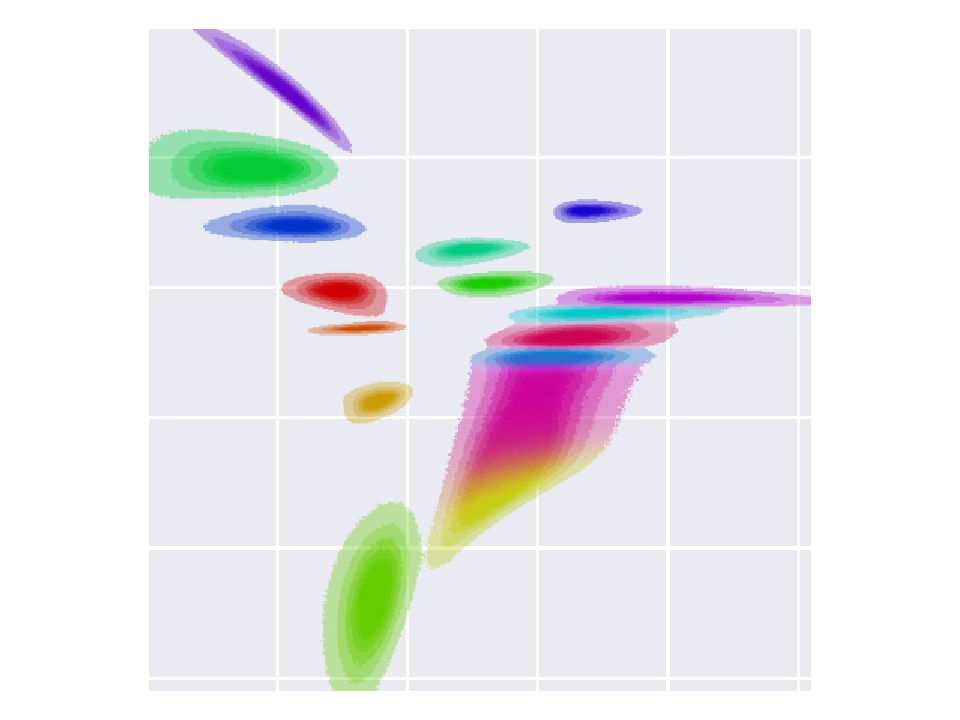
\includegraphics[width=0.225\textwidth]{figures/experiments_figures/latent_space/set_modeling/layer_reverse_07.pdf}  & 
            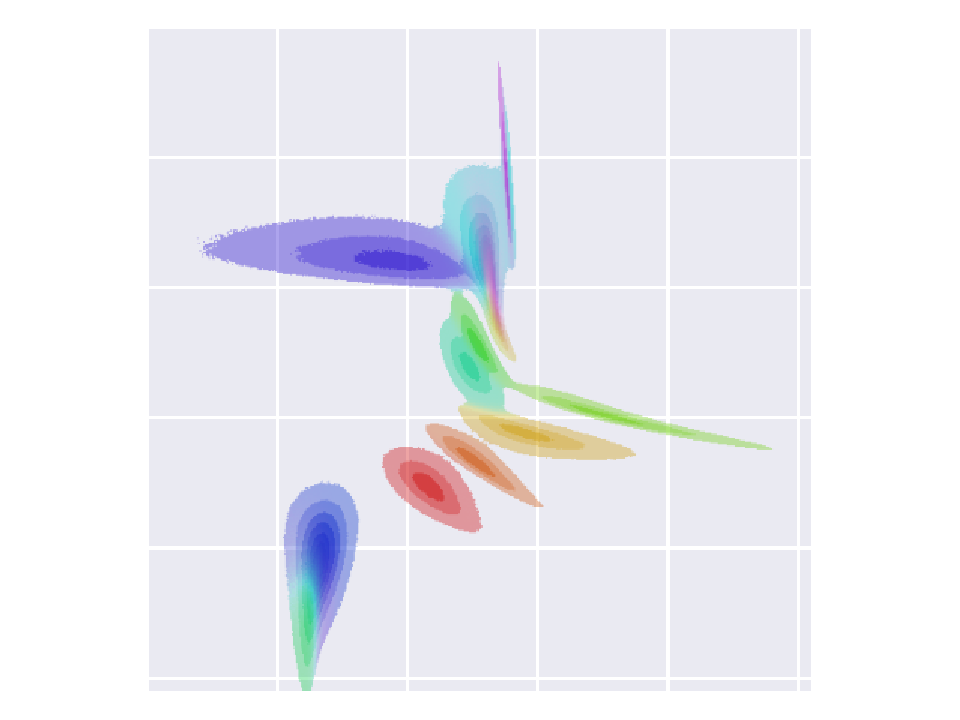
\includegraphics[width=0.225\textwidth]{figures/experiments_figures/latent_space/set_modeling/layer_reverse_04.pdf}  & 
            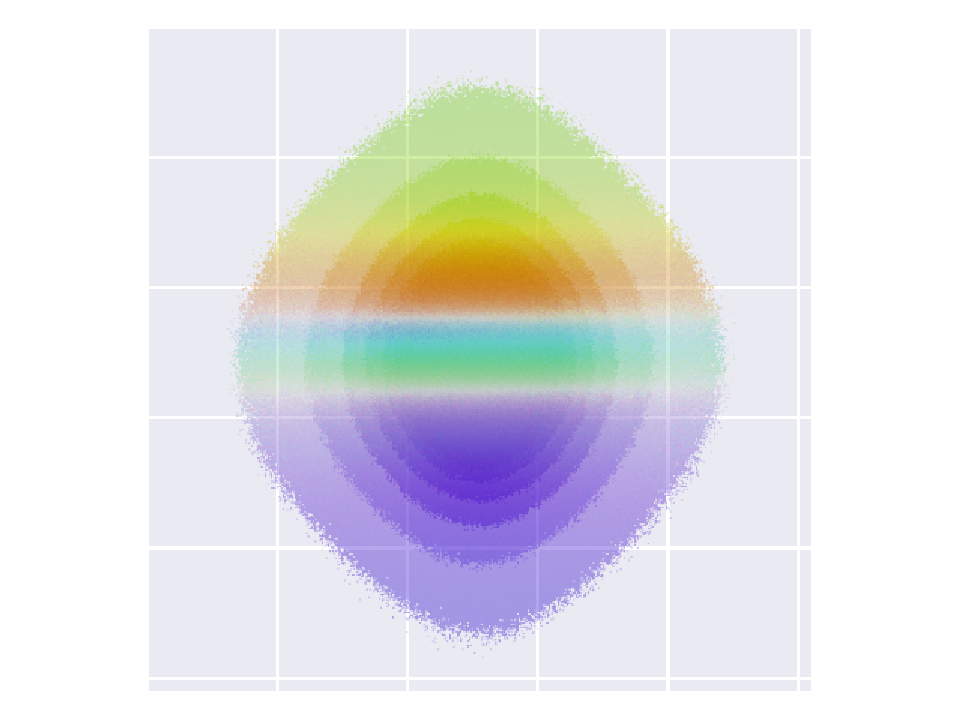
\includegraphics[width=0.225\textwidth]{figures/experiments_figures/latent_space/set_modeling/layer_reverse_01.pdf}
            \\
            \multicolumn{4}{c}{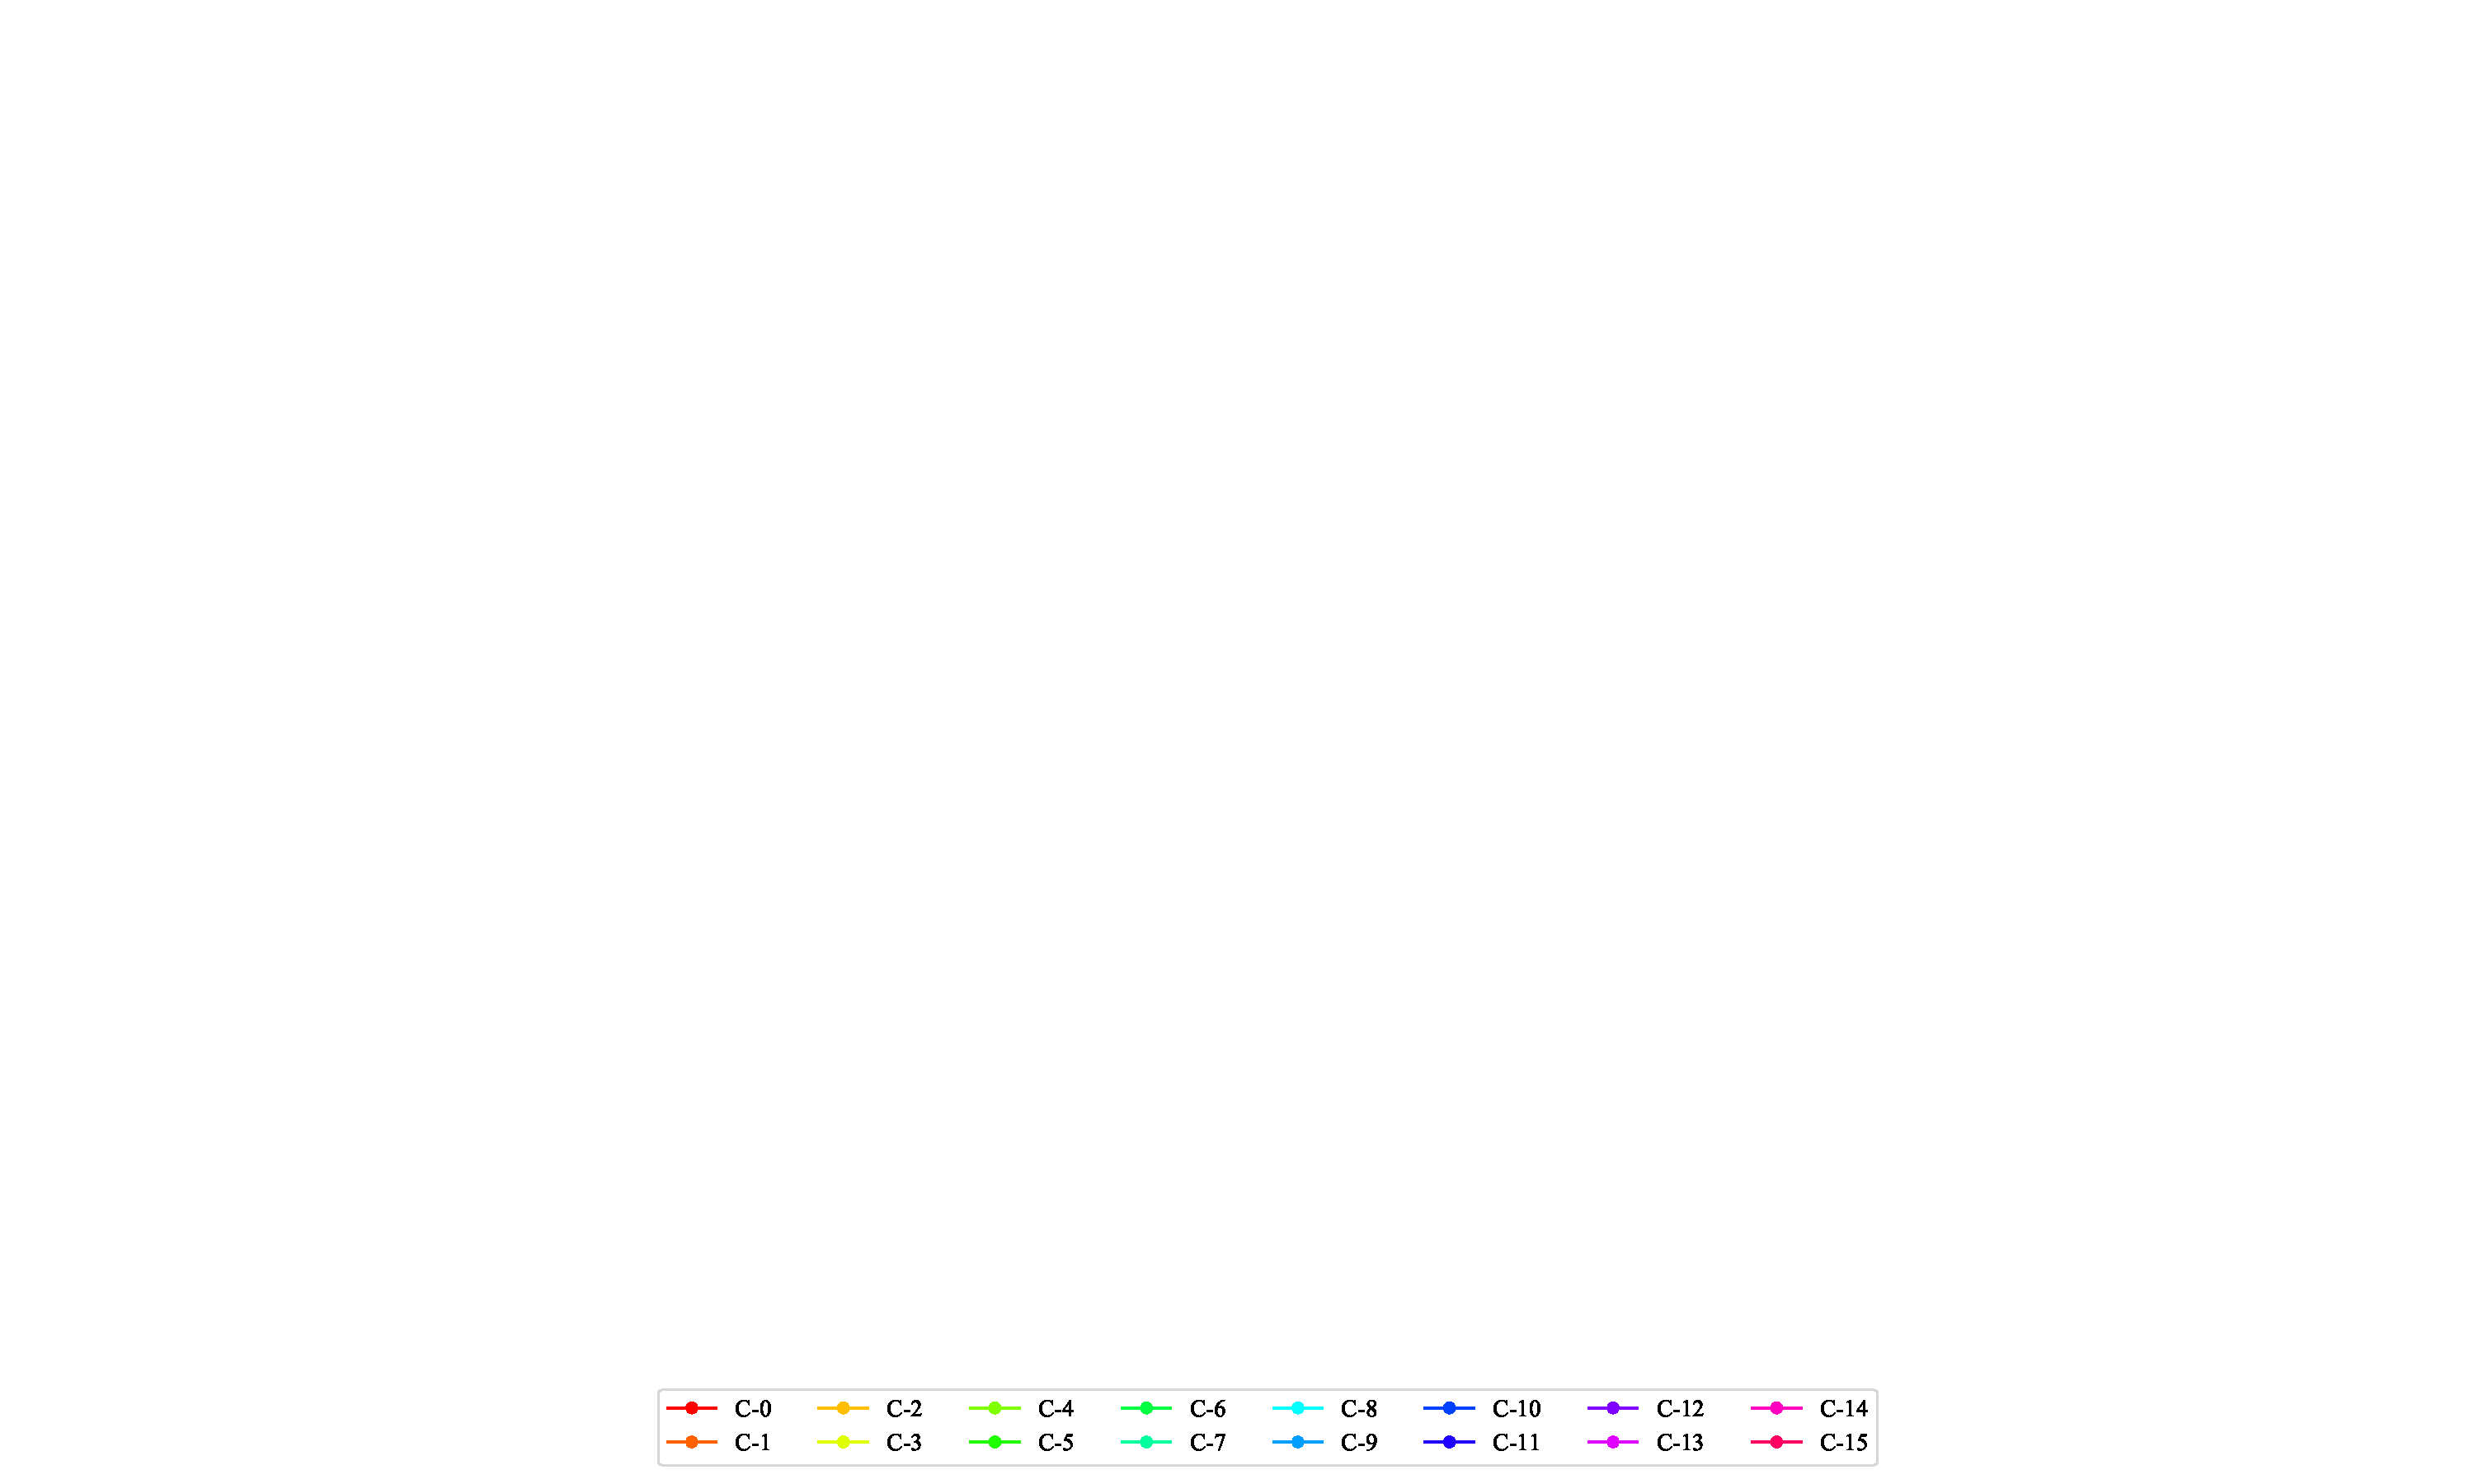
\includegraphics[width=0.95\textwidth]{figures/experiments_figures/latent_space/set_modeling/legend_visu.pdf}}\\
        \end{tabular}
        \caption{Reverse sampling\\[0.2cm]}
    \end{subfigure}
    \caption[Latent space of set modeling flow]{Visualization of the latent space in a 4-layer flow trained on set modeling with 16 categories (best viewed in color and digital).
    The illustration follows the same setup as Figure~\ref{fig:experiments_discussion_latent_space_graph_coloring}.
    The legend beneath the latent space visualization show the color assignment for the 16 categories $C_{0}$ to $C_{15}$.}
    \label{fig:experiments_discussion_latent_space_set}
\end{figure}

To show the effect of more categories, we also visualize the latent space of a Categorical Normalizing Flow trained on set modeling in Figure~\ref{fig:experiments_discussion_latent_space_set}. 
We can see that some categories are combined at different stages throughout the flow. 
As there are no clear relations among the categories, the decision of which categories to combine when is arbitrary and changes across seeds.
Similarly to the base distribution in graph coloring, we experience a clear separation of categories in the logistics.
Again, those colors are not pure and any category can be created based on any of sample in the logistic.
Note that the visually larger purple part is due to the combination of categories with similar colors ($C_{10}, C_{11}, C_{12}$, and $C_{13}$) and not because of a larger probability density of a single category.

In conclusion, the visualization of the latent space shows that:
\begin{itemize}
    \item The transformation flexibility provided by the continuous space is used to partly merge densities of different categories. For instance in graph coloring, the probability density of green and red are merged in the first flows for those nodes that can have any of the two colors without breaking the validity constraint (for example, see Figure~\ref{fig:experiments_graph_coloring_examples}a, bottom right node). 
    Meanwhile, other variables stay with a unique category.
    This merge process happens throughout the flow at different stages, until all categories have been merged into the base distribution.
    \item The continuous base distribution is split into areas of dominant colors. Such a separation can help to influence the categorical output during sampling, for instance when we are looking for a certain output. 
    This can be particularly of interest for applications like drug discovery and property optimization which work on latent generative models.
    \item Looking at the latent space allows us to interpret the model. With a sufficient number of samples, the probability density per category can be visualized throughout the flow and shows how the model maps the mixture model back to the base distribution. Furthermore, the merging process shows the interactions among categories that are modeled by the flow.
\end{itemize}

\subsubsection{Comparison to Discrete Normalizing Flows}

One of the key aspects of Categorical Normalizing Flows' expressiveness is the flexible transformations in continuous space. 
As seen in the last subsection, the flow often combines parts of probability densities of two or more categories while other parts stay separated.
Such transformations seem to be crucial for modeling categorical distributions.
In contrast, Discrete Normalizing Flows do not allow such transformation.
Due to the invertibility constrain in discrete space, categories can only be permuted or combined by an equal ratio (i.e. two categories can be mapped to the same output by a coupling layer if the input contains the information which category it is). 
Stochastic combinations or ones with flexible weights would break the invertibility because instead of probability densities, categories are represented by a single number. 
This limits Discrete Normalizing Flows in becoming universal (i.e. being able to learn any input distribution) as continuous normalizing flows are.

Nevertheless, representing categories by a single number has one decisive advantage: the input is always the same for a discrete data point.
When training Categorical Normalizing Flows, the first step is to sample from the encoding distribution $\tilde{\bm{z}}\sim q(\bm{z}|\bm{x})$, which will be different every time we sample.
To learn the true categorical distribution, the flow has to model an (optimal) transformation for each continuous data point. 
This variation in the input increases computation and time needed for training considerably.
For instance, when we compare the training speed of the LSTM baseline with the autoregressive Categorical Normalizing Flow on language modeling (text8 dataset), the flow takes almost 5 times as many iterations to obtain the same performance as the baseline.
Similarly, on simple datasets like set shuffling, a considerable amount of optimization steps are necessary to achieve the close-to-optimal performance (about 100k iterations) although there is little variation in the categorical dataset. 
The phenomenon of long training times for continuous normalizing flows has also been found on image modeling \cite{VFlow, Flow++}.

Therefore, a future direction would be to combine the benefits of a discrete input with the flexible transformations of Categorical Normalizing Flows.
One possibility to do so is to introduce stochastic layers into the normalizing flows \cite{StochasticNF, SurVAE}.
While this breaks the initial invertibility assumption of normalizing flows, it uses variational inference with a similar idea as the encoding distribution of Categorical Normalizing Flows. 
Especially the idea of surjective flows by \citet{SurVAE}, where only the forward direction of a flow layer is deterministically invertible while the reverse is stochastic, can be an interesting direction for Discrete NFs.
However, it should be kept in mind that Discrete Normalizing Flows have also the disadvantage of differentiating through discrete operators which introduce additional, considerable challenges.
Thus, we leave this idea as a potential starting point for future work.
% IDEA: We can express an autoregressive model as surjective discrete NF

% \begin{itemize}
%     \item Discuss in more detail the variational encoding (paragraph conclusion)
%     \item Visualize the latent space and its transitions (check graph coloring and set modeling)
%     \item GraphCNF (permutation invariance)
%     \begin{itemize}
%         \item GraphCNF is more memory intensive and requires more parameters. RNNs on the other hand are slow in sampling. If sampling is not a major priority and an "optimal" order is known, RNN might work well. In other cases and more general, GraphCNF is the better choice.
%     \end{itemize}
%     \item General continuous normalizing flows
%     \begin{itemize}
%         \item One current limitation of continuous flows is the training speed. While purely autoregressive models can learn simple categorical distributions within a few iterations, normalizing flows take much longer. Even if NFs are autoregressive.
%         We found that this noise can be helpful and acts as a regularizer for small datasets as it has been the case for the Penn Treebank in the language experiments. 
%         On the other hand, this sampling noise is not there anymore in Discrete Normalizing Flows. 
%         Possible future direction: combine flexibility of Categorical NF with "discreteness" of Discrete NFs 
%     \end{itemize}
%     \item 
% \end{itemize}